%% Bản tiếng Việt song song của main.tex: cùng cấu trúc, cùng số định lý, hình và công thức.
%% Chỉ dùng để đọc đối chiếu. Không nộp bản này.
%% Biên dịch: pdflatex main-vi && bibtex main-vi && pdflatex main-vi && pdflatex main-vi

\documentclass[pdflatex,sn-mathphys-num]{sn-jnl}
\usepackage{etoolbox}
\makeatletter
\patchcmd{\@maketitle}{Contributing authors:}{E-mail(s):}{}{\PackageWarning{main-vi}{author label patch failed}}
\makeatother

%% Tiếng Việt cần mã hóa T5 và đầu vào UTF-8; \k dùng cho tên Gąsieniec trong tài liệu tham khảo.
\usepackage[T1,T5]{fontenc}%
\DeclareTextCommandDefault{\k}[1]{{\fontencoding{T1}\selectfont\k{#1}}}%
\usepackage[utf8]{inputenc}%
\usepackage{graphicx}%
\usepackage{multirow}%
\usepackage{amsmath,amssymb,amsfonts}%
\usepackage{amsthm}%
\usepackage{mathrsfs}%
\usepackage[title]{appendix}%
\usepackage{xcolor}%
\usepackage{textcomp}%
\usepackage{manyfoot}%
\usepackage{booktabs}%
\usepackage{algorithm}%
\usepackage{algorithmicx}%
\usepackage{algpseudocode}%
\usepackage{tikz}%
\usepackage{pgfplots}%
\pgfplotsset{compat=1.18}%
\usetikzlibrary{arrows.meta,calc,positioning,backgrounds}%

\theoremstyle{thmstyleone}%
\newtheorem{theorem}{Định lý}%
\newtheorem{lemma}[theorem]{Bổ đề}%
\newtheorem{proposition}[theorem]{Mệnh đề}%
\newtheorem{corollary}[theorem]{Hệ quả}%
\theoremstyle{thmstyletwo}%
\newtheorem{example}{Ví dụ}%
\newtheorem{remark}{Nhận xét}%
\theoremstyle{thmstylethree}%
\newtheorem{definition}{Định nghĩa}%

\renewcommand{\proofname}{Chứng minh}%
\renewcommand{\abstractname}{Tóm tắt}%
\renewcommand{\refname}{Tài liệu tham khảo}%
\renewcommand{\figurename}{Hình}%
\renewcommand{\tablename}{Bảng}%
\floatname{algorithm}{Thuật toán}%
\algrenewcommand\algorithmicwhile{\textbf{khi}}
\algrenewcommand\algorithmicdo{\textbf{làm}}
\algrenewcommand\algorithmicif{\textbf{nếu}}
\algrenewcommand\algorithmicthen{\textbf{thì}}
\algrenewcommand\algorithmicend{\textbf{hết}}
\algrenewcommand\algorithmicreturn{\textbf{trả về}}

\newcommand{\N}{\mathbb{N}}
\newcommand{\Z}{\mathbb{Z}}
\newcommand{\cE}{\mathcal{E}}
\newcommand{\cB}{\mathcal{B}}
\newcommand{\e}{\mathbf{e}}
\newcommand{\out}{\mathrm{out}}
\newcommand{\inn}{\mathrm{in}}
\newcommand{\IN}{\mathrm{IN}}
\newcommand{\OUT}{\mathrm{OUT}}
\newcommand{\FIX}{\textup{\textsc{Fix}}}
\newcommand{\FREE}{\textup{\textsc{Free}}}
\newcommand{\ENDSET}{\textup{\textsc{EndSet}}}
\newcommand{\SFIX}{\textup{\textsc{Strict-Fix}}}
\newcommand{\SFREE}{\textup{\textsc{Strict-Free}}}
\newcommand{\abs}[1]{\lvert #1\rvert}
\newcommand{\floor}[1]{\lfloor #1\rfloor}
\newcommand{\YES}{\texttt{YES}}
\newcommand{\NO}{\texttt{NO}}

%% Bảng màu thân thiện với người mù màu (Okabe--Ito). Mỗi màu đi kèm kiểu nét,
%% nên hình vẫn đọc được khi in đen trắng.
\definecolor{cA}{HTML}{0072B2}
\definecolor{cB}{HTML}{D55E00}
\definecolor{cTa}{HTML}{009E73}
\definecolor{cTb}{HTML}{E69F00}
\tikzset{
  >={Stealth[length=4.5pt,width=3.6pt]},
  vtx/.style={circle,draw,semithick,fill=white,minimum size=5.6mm,inner sep=0pt,font=\small},
  svtx/.style={circle,draw,semithick,fill=white,minimum size=5.4mm,inner sep=0pt,font=\footnotesize},
  port/.style={circle,draw,semithick,fill=white,minimum size=2.4mm,inner sep=0pt},
  tlab/.style={fill=white,inner sep=1pt,font=\scriptsize,text=black},
  cnt/.style={rectangle,rounded corners=1pt,draw,thin,fill=white,inner sep=1.5pt,font=\scriptsize},
  sub/.style={font=\footnotesize},
  note/.style={font=\scriptsize,text=black!70,align=left},
  t1/.style={cTa,very thick},
  t2/.style={cTb,very thick,densely dashed},
  walkA/.style={cA,very thick,->},
  walkB/.style={cB,very thick,->,densely dashed},
}
\newcommand{\RunningVertices}{%
  \node[vtx] (x) at (0,0) {$x$};
  \node[vtx] (u) at (1.45,0) {$u$};
  \node[vtx] (y) at (2.9,0) {$y$};
  \node[vtx] (v) at (0.8,1.3) {$v$};
  \node[vtx] (w) at (2.1,1.3) {$w$};}

\raggedbottom

\begin{document}

\title[Phủ chính xác cạnh bằng walk thời gian]{Phủ chính xác cạnh bằng walk thời gian chặt và không chặt}

\author[1]{\fnm{Duc Thien} \sur{Quach}}\email{thienchy3305@gmail.com}

\author*[1]{\fnm{Manh Cuong} \sur{Tran}}\email{tranmanhcuong@vnu.edu.vn}

\affil[1]{\orgdiv{Khoa Công nghệ Thông tin}, \orgname{Trường Đại học Công nghệ, Đại học Quốc gia Hà Nội}, \orgaddress{\city{Hà Nội}, \country{Việt Nam}}}

\abstract{Cho một đồ thị thời gian vô hướng và số walk xuất phát tại mỗi đỉnh, bài toán phủ chính xác cạnh hỏi liệu các cạnh có thể được chia thành các walk thời gian với đỉnh kết thúc cho trước hoặc tự do hay không. Với walk không chặt, tức các walk có nhãn thời gian không bao giờ giảm, Deligkas và cộng sự đã khẳng định tại AAAI 2025 rằng bài toán giải được trong thời gian đa thức, thông qua một phép quy về đồ thị tĩnh; một phản ví dụ năm đỉnh cho thấy phép quy này, xây dựng như Hình 3 của họ, bỏ sót một điều kiện. Chúng tôi đưa ra một chứng minh đầy đủ tính đa thức bằng một con đường khác, dựa trên luồng submodular M-lồi. Một định hướng là khả thi khi và chỉ khi một điều kiện đếm được thỏa mãn và mọi thành phần snapshot đều chứa một walk; chỉ các thành phần có bậc và bộ đếm walk đều chẵn mới có thể vi phạm điều kiện thứ hai. Đếm walk theo cặp, chúng tôi chứng minh tập trạng thái của một thành phần như vậy vẫn là M-lồi sau khi bỏ trạng thái chết, điều này cho một mô hình luồng submodular M-lồi và một thuật toán đường tăng trả về các walk hoặc một chứng nhận vô nghiệm. Với walk chặt, tức các walk có nhãn thời gian tăng nghiêm ngặt, chúng tôi chứng minh bài toán NP-đầy đủ ngay cả khi đỉnh kết thúc được cho trước và có sáu nhãn thời gian, giải quyết một trường hợp còn mở do Deligkas và cộng sự nêu. Các thực nghiệm trên instance có tới $387{,}467$ cạnh phù hợp với tính đúng của cài đặt và cho thấy hiệu năng trên các bộ thử đã chọn.}

\keywords{Đồ thị thời gian, Phủ chính xác cạnh, Walk thời gian, Tập M-lồi, Luồng submodular, NP-đầy đủ}

\pacs[MSC Classification]{05C85, 90C27, 90C35, 68Q17}

\maketitle

%% =====================================================================

\section{Giới thiệu}\label{sec:intro}

Đồ thị thời gian mô hình hóa các kết nối phụ thuộc thời gian trong mạng tiếp xúc, mạng truyền thông và mạng giao thông~\cite{kempe2002,holme2012,casteigts2012,michail2016}. Phủ các cạnh của mạng bằng các lộ trình là vấn đề trung tâm của bài toán người đưa thư Trung Hoa và định tuyến cung~\cite{edmonds1973,corberan2015}, còn việc phân công các chuyến theo lịch cho phương tiện bổ sung các ràng buộc thời gian~\cite{dantzig1954,bunte2009,kliewer2006}. Phủ chính xác cạnh bằng walk thời gian hỏi liệu các cạnh mang nhãn thời gian có thể được chia thành các walk tôn trọng thời gian, với số walk xuất phát tại mỗi đỉnh được cho trước, hay không.

Deligkas và cộng sự~\cite{deligkas2025} giới thiệu bài toán phủ chính xác cạnh trong đồ thị thời gian (arXiv 2024; AAAI 2025). Chúng tôi nghiên cứu trường hợp vô hướng với các đỉnh xuất phát cho trước và các đỉnh kết thúc cho trước hoặc tự do. Chiều của mỗi lần đi qua cạnh là một phần của lời giải. Chúng tôi xét cả walk \emph{không chặt}, có nhãn thời gian không giảm, và walk \emph{chặt}, có nhãn thời gian tăng nghiêm ngặt. Mô hình không chặt cho phép các cạnh liên tiếp có cùng nhãn thời gian khi các sự kiện được ghi lại với độ phân giải thời gian hữu hạn. Sự phân biệt này có thể làm thay đổi độ phức tạp của các bài toán đồ thị thời gian~\cite{casteigts2024}. Deligkas và cộng sự chứng minh tính NP-đầy đủ cho walk không có đỉnh xuất phát cho trước, tương ứng với việc cực tiểu hóa số walk chứ không phải các bài toán của chúng tôi với số lượng xuất phát cho trước, và để mở trường hợp tổng quát của walk chặt với đầu cuối cho trước~\cite{deligkas2025}.

Phép quy tĩnh mà Deligkas và cộng sự dùng để lập luận về tính giải được trong thời gian đa thức cho walk không chặt bỏ sót một điều kiện cần: mọi thành phần liên thông chứa cạnh trong một \emph{snapshot}, tức đồ thị con gồm các cạnh có cùng nhãn thời gian, phải chứa một walk ngay trước thời điểm đó. Phản ví dụ của chúng tôi vô nghiệm về mặt thời gian, dù đồ thị tĩnh của nó có một phủ chính xác cạnh. Mục~\ref{sec:counterexample} trình bày cách xây dựng.

\paragraph{Đóng góp.} Các đóng góp của chúng tôi, cùng các kết quả chứng minh chúng, như sau.
\begin{enumerate}
\item \emph{Đặc trưng.} Một định hướng của các cạnh khả thực hiện bởi các walk khi và chỉ khi điều kiện đếm được thỏa mãn và mọi thành phần snapshot đều chứa một walk (Định lý~\ref{thm:char}). Chỉ các thành phần chẵn mới có thể vi phạm điều kiện thứ hai (Bổ đề~\ref{lem:noneven}), nên các instance không có chúng được giải bằng một luồng cực đại (Hệ quả~\ref{cor:flow}).
\item \emph{Tính M-lồi của thành phần chẵn.} Bằng cách đếm walk theo cặp, chúng tôi chứng minh rằng tập trạng thái của một thành phần chẵn vẫn M-lồi sau khi bỏ trạng thái chết (Bổ đề~\ref{lem:gamma}(b)). Đây là kết quả cấu trúc mới then chốt.
\item \emph{Chứng minh đầy đủ cho walk không chặt.} Deligkas và cộng sự khẳng định tính đa thức; phép quy tĩnh của họ không nắm bắt điều kiện tồn tại walk (Mục~\ref{sec:counterexample}), nên chúng tôi đưa ra một chứng minh độc lập: bài toán là một bài toán luồng submodular M-lồi (Định lý~\ref{thm:reduction}). Thuật toán đường tăng của chúng tôi trả về các walk hoặc một chứng nhận vô nghiệm (Định lý~\ref{thm:correct}) trong thời gian đa thức (Định lý~\ref{thm:time}) và mở rộng cho trường hợp đỉnh kết thúc bị giới hạn trong một tập cho trước (Định lý~\ref{thm:endset}).
\item \emph{Tính NP-đầy đủ cho walk chặt.} Bài toán chặt là NP-đầy đủ ngay cả khi đỉnh kết thúc được cho trước và chỉ có sáu nhãn thời gian (Định lý~\ref{thm:strict}), qua đó giải quyết trường hợp được để mở trong~\cite{deligkas2025}.
\item \emph{Phép quy tĩnh.} Chúng tôi đưa ra phản ví dụ năm đỉnh (Mệnh đề~\ref{prop:aaai}) và chỉ ra chính xác những ràng buộc định hướng mà đồ thị tĩnh biểu diễn (Bổ đề~\ref{lem:aaai}).
\end{enumerate}
Các thực nghiệm tính toán (Mục~\ref{sec:eval}) ủng hộ tính đúng và tính thực dụng của thuật toán trên instance tổng hợp, dữ liệu tiếp xúc và thời gian biểu giao thông có tới $387.467$ cạnh.

Mục~\ref{sec:prelim} định nghĩa các bài toán và điểm lại các công trình liên quan. Mục~\ref{sec:char} và~\ref{sec:counterexample} thiết lập đặc trưng định hướng và phân tích phép quy tĩnh. Mục~\ref{sec:mconvex} và~\ref{sec:method} phát triển mô hình M-lồi và thuật toán. Mục~\ref{sec:strict} chứng minh tính NP-đầy đủ cho walk chặt, Mục~\ref{sec:eval} báo cáo thực nghiệm, và Mục~\ref{sec:conclusion} kết luận.

%% =====================================================================
\section{Phát biểu bài toán và công trình liên quan}\label{sec:prelim}

\subsection{Phát biểu bài toán}\label{sec:problem}

Ta ký hiệu $\N=\{0,1,2,\ldots\}$ và dùng $\Z$ cho tập số nguyên. Một đồ thị thời gian vô hướng là một bộ ba $G=(V,\cE,\tau)$, trong đó $V$ là tập đỉnh, $\cE$ là tập cạnh và $\tau:\cE\to\N$ gán một nhãn thời gian cho mỗi cạnh. Ta ký hiệu $n=\abs{V}$ và $m=\abs{\cE}$. Các cạnh song song được cho phép và được xem là các phần tử phân biệt của $\cE$, nhưng không cho phép khuyên. Với mỗi thời điểm $t$, đặt $E_t=\{e\in\cE:\tau(e)=t\}$ và gọi $G_t=(V,E_t)$ là \emph{snapshot} tương ứng. Trong suốt bài báo, một thành phần của snapshot là một thành phần liên thông chứa ít nhất một cạnh.

Một \emph{walk thời gian không chặt} là một dãy xen kẽ
\[
  W=(v_0,e_1,v_1,\ldots,e_\ell,v_\ell)
\]
trong đó $e_i$ có hai đầu mút $v_{i-1}$ và $v_i$ với $i=1,\ldots,\ell$, và $\tau(e_1)\le\cdots\le\tau(e_\ell)$. Đỉnh xuất phát và đỉnh kết thúc của nó là $v_0$ và $v_\ell$. Một walk rỗng có $\ell=0$ và chỉ gồm một đỉnh. Mặc dù một walk nói chung có thể lặp lại cạnh, phủ chính xác cạnh yêu cầu mỗi cạnh được đi qua đúng một lần trên toàn bộ các walk.

Hai bài toán quyết định chính cho trước một vector $a\in\N^V$ gồm số lượng xuất phát, với $k=\sum_v a_v$. Chúng tôi cũng xét một biến thể giới hạn tập đỉnh kết thúc.

\begin{definition}\label{def:problems}
\begin{itemize}
\item \FREE{}: quyết định liệu có tồn tại $k$ walk thời gian không chặt cùng nhau đi qua mỗi cạnh của $\cE$ đúng một lần, với đúng $a_v$ walk xuất phát tại mỗi đỉnh $v$, hay không.
\item \FIX{}: cho thêm một vector $z\in\N^V$, quyết định liệu có tồn tại các walk thỏa mãn \FREE{} với đúng $z_v$ walk kết thúc tại mỗi đỉnh $v$, hay không.
\item \ENDSET{}: như \FREE{}, với yêu cầu mọi walk kết thúc trong một tập $T\subseteq V$ cho trước.
\end{itemize}
\end{definition}

Trong \FIX{}, các vector $a$ và $z$ cho trước số walk xuất phát và kết thúc, nhưng không chỉ định đỉnh xuất phát nào được ghép với đỉnh kết thúc nào. Trừ khi có phát biểu khác, các walk đều không chặt.

Các cận thời gian chạy đếm phép toán số học trong mô hình chi phí đơn vị cho các số nguyên có kích thước một từ máy, bao gồm các số lượng đầu vào $a_v$ và $z_v$. Chúng không phải là các cận độ phức tạp bit. Với bội số được mã hóa nhị phân, việc liệt kê tường minh mọi walk rỗng có thể đòi hỏi đầu ra có kích thước tăng theo hàm mũ của độ dài đầu vào. Vì vậy chúng tôi trả về một lời giải \emph{nén}: danh sách các walk không rỗng và số walk rỗng tại mỗi đỉnh.

\subsection{Công trình liên quan}\label{sec:related}

\paragraph{Phủ chính xác cạnh trong đồ thị thời gian.}
Deligkas và cộng sự~\cite{deligkas2025} nghiên cứu phủ chính xác cạnh bằng đường đi, đường (trail) và walk thời gian. Với walk chặt có đầu cuối cố định, Hệ quả~6.4 của họ xử lý đồ thị thời gian proper, trong đó mỗi snapshot là một ghép cặp. Định lý~6.5 của họ đưa ra một thuật toán $O(2^k k\,t_{\max})$ khi $\abs{E_t}\in\{0,k\}$ tại mọi thời điểm, trong đó $k$ là số walk cho trước và $t_{\max}$ là nhãn thời gian lớn nhất. Với đồ thị thời gian có hướng, Định lý~6.1 của họ cho tính giải được trong thời gian đa thức cho walk không chặt với đầu cuối xuất phát cho trước, còn Định lý~5.2 đưa ra một thuật toán thời gian tuyến tính cho walk chặt khi dòng cạnh được cung cấp theo thứ tự thời gian. Mệnh đề~5.1 đưa ra một thuật toán $n^{O(k)}$ cho $k$ walk.

Kết quả đa thức cho trường hợp không chặt của họ, Định lý~6.3, chỉ đề cập đến đầu cuối xuất phát, trong khi phác thảo chứng minh và Hình~3 của nó cũng dùng đầu cuối kết thúc. Phiên bản mở rộng~\cite{deligkas2024arxiv} phát biểu kết quả cho đầu cuối xuất phát và kết thúc cho trước. Mục~\ref{sec:counterexample} phân tích cách xây dựng theo các cách đọc này về đầu cuối.

Phản ví dụ ở Mục~\ref{sec:counterexample} là một đồ thị đơn, và phép xây dựng khó ở Mục~\ref{sec:strict} không có cạnh song song trong một snapshot.

\paragraph{Mạng thời gian và các bài toán phủ.}
Biểu diễn bằng các bản sao theo thời gian là cách biểu diễn chuẩn trong đồ thị thời gian~\cite{kostakos2009} và các bài toán luồng thời gian~\cite{akrida2019}. Mạng chuỗi và mạng cổng của chúng tôi bổ sung các ràng buộc chi phối việc định hướng và phủ các cạnh của snapshot. Các bài toán phủ thời gian liên quan yêu cầu một walk duy nhất đi qua mọi cạnh tĩnh~\cite{marino2023}, khám phá mọi cạnh~\cite{bumpus2023}, hoặc phủ các đỉnh của một đồ thị có hướng không chu trình (DAG) thời gian bằng đường đi~\cite{chakraborty2024}.

\paragraph{Tính lồi rời rạc và định hướng.}
Mô hình của chúng tôi dựa trên tập M-lồi, luồng submodular M-lồi~\cite{edmonds1977,murota1999,murota2003,fujishige2005} và định hướng với ràng buộc bậc~\cite{hakimi1965,frank2011}. Các thuật toán luồng submodular tổng quát cho tính giải được trong thời gian đa thức. Chúng tôi dùng lược đồ đường tăng chuẩn~\cite{fujishige2005} với các phép kiểm tra trao đổi tổ hợp. Kiến thức nền liên quan gồm định hướng với ràng buộc chẵn lẻ~\cite{frank2011}, định hướng liên thông mạnh và mạng nguyên~\cite{abdi2025}, và hệ nhảy~\cite{bouchet1995}.

%% =====================================================================
\section{Đặc trưng của các định hướng khả thi}\label{sec:char}

Chúng tôi đặc trưng hóa các định hướng khả thi và quy khó khăn còn lại về các thành phần chẵn của snapshot.

\subsection{Định hướng và bộ đếm walk}

Một walk đi qua cạnh $\{u,v\}$ từ $u$ đến $v$ \emph{định hướng} nó thành $u\to v$, và $u$ được gọi là \emph{đuôi}. Một lời giải do đó cảm sinh một định hướng của mọi cạnh. Với một định hướng, gọi $\out_t(v)$ và $\inn_t(v)$ lần lượt là số cung của $E_t$ có đuôi $v$ và có đầu $v$. \emph{Bộ đếm walk} $c_t(v)$ là số walk tại $v$ ngay trước thời điểm $t$. Bộ đếm bắt đầu từ $a_v$ và tiến hóa theo
\[
  c_{t^+}(v)=c_t(v)-\out_t(v)+\inn_t(v),
\]
trong đó $t^+$ là thời điểm ngay sau $t$. Tính chẵn lẻ của bộ đếm được xác định bởi $a_v$ cộng số cạnh kề với $v$ trước $t$, không phụ thuộc vào định hướng.

Gọi $t_{v,1}<\dots<t_{v,q_v}$ là các nhãn thời gian mà $v$ có cạnh kề (các \emph{lần xuất hiện} của $v$), gọi $g_{v,j}$ là bậc của $v$ trong $E_{t_{v,j}}$, và đặt $G_{v,j}=\sum_{i\le j}g_{v,i}$ và $G_v=G_{v,q_v}$. Với một định hướng, gọi $b_{v,j}$ là số cung của $E_{t_{v,j}}$ có đuôi $v$ và $B_{v,j}=\sum_{i\le j}b_{v,i}$, trong đó tổng rỗng bằng không. Với \FIX{}, chúng tôi đặt $h_v=(a_v+G_v-z_v)/2$, là số cung có đuôi $v$ trong mọi lời giải, được xác định bởi số walk cuối cùng $z_v$.

\begin{theorem}\label{thm:char}
Một định hướng là khả thi bởi các walk xuất phát theo $a$ (bài toán \FREE{}) khi và chỉ khi, tại mọi thời điểm $t$,
\begin{enumerate}
\item[(i)] $\out_t(v)-\inn_t(v)\le c_t(v)$ với mọi đỉnh $v$, và
\item[(ii)] mọi thành phần snapshot $K$ của $E_t$ đều chứa một walk, tức là $\sum_{v\in K}c_t(v)\ge 1$.
\end{enumerate}
Với \FIX{}, điều kiện bổ sung là số walk cuối cùng tại $v$ bằng $z_v$ với mọi $v$, tức là $B_{v,q_v}=h_v$.
\end{theorem}

\begin{proof}
\emph{Điều kiện cần.} Tại thời điểm $t$, mọi walk rời khỏi $v$ hoặc đã ở $v$ trước $t$ hoặc đến $v$ trong lúc $t$, nên $\out_t(v)\le c_t(v)+\inn_t(v)$, đó là (i). Các cạnh mà một walk dùng tại thời điểm $t$ tạo thành một đường (trail) trong một thành phần $K$ của $E_t$, và walk nằm tại đỉnh đầu tiên của đường này ngay trước $t$. Do đó mọi thành phần có cạnh đều chứa một walk. Với \FIX{}, số walk cuối cùng tại $v$ là $a_v+G_v-2B_{v,q_v}=z_v$.

\emph{Điều kiện đủ.} Ta xử lý các thời điểm theo thứ tự tăng dần và các thành phần của $E_t$ một cách độc lập. Gọi $\vec K$ là đồ thị có hướng của $K$ và $r=\sum_{v\in K}\max(0,\out_t(v)-\inn_t(v))$. Nếu $r>0$, thêm $r$ cung giả từ các đỉnh có $\inn>\out$ đến các đỉnh có $\out>\inn$ để mọi đỉnh cân bằng. Đồ thị thu được liên thông yếu và cân bằng, nên có chu trình Euler. Bỏ các cung giả sẽ cắt chu trình thành $r$ đường, và đúng $\out_t(v)-\inn_t(v)$ đường trong số đó bắt đầu tại mỗi đỉnh $v$ có thặng dư. Theo (i), $v$ có đủ walk để đi các đường này. Nếu $r=0$ thì $\vec K$ là Euler. Theo (ii) có một đỉnh của $K$ đang giữ một walk, và walk này đi theo một chu trình Euler xuất phát từ đỉnh đó. Mọi walk khác đứng chờ. Số walk tại mỗi đỉnh sau $t$ bằng $c_{t^+}$, nên quy nạp tiếp tục. Với \FIX{}, số cuối cùng là $z$.
\end{proof}

Chứng minh điều kiện đủ cho một thuật toán $O(n+m)$, sau khi sắp xếp các cạnh, xây dựng các walk từ một định hướng thỏa mãn (i) và (ii) bằng thuật toán Hierholzer~\cite{hierholzer1873}.

\begin{corollary}\label{cor:directed}
Nếu chiều của mọi cạnh được cho và walk phải đi theo chiều đó, thì \FREE{} và \FIX{} được quyết định trong thời gian $O(n+m\log(m+1))$.
\end{corollary}

\begin{proof}
Định hướng đã cố định, nên theo Định lý~\ref{thm:char} chỉ cần kiểm tra (i), (ii) và, với \FIX{}, điều kiện đầu cuối. Sau khi sắp xếp các cạnh theo thời gian, một lượt duyệt qua các snapshot tính mọi bộ đếm và thành phần.
\end{proof}

Hệ quả~\ref{cor:directed} bao quát các instance có chiều cho trước, chẳng hạn các thời gian biểu giao thông. Khó khăn còn lại nằm ở việc chọn chiều.

\subsection{Thành phần chẵn và mạng chuỗi}

\begin{definition}\label{def:even}
Một thành phần snapshot $K$ của $E_t$ là \emph{chẵn} nếu mọi đỉnh của $K$ có bậc chẵn trong $E_t$ và bộ đếm walk $c_t$ chẵn. Một thành phần chẵn là \emph{chết} dưới một định hướng nếu $c_t(v)=0$ với mọi $v\in K$.
\end{definition}

Hai cạnh song song và một tam giác có bộ đếm walk chẵn là các thành phần chẵn. Một đường đi không chẵn vì hai đầu của nó có bậc lẻ.

\begin{lemma}\label{lem:noneven}
Nếu một định hướng thỏa mãn (i) và thành phần snapshot $K$ của $E_t$ không chẵn, thì $K$ thỏa mãn (ii).
\end{lemma}

\begin{proof}
Nếu có đỉnh của $K$ có bậc lẻ trong $E_t$, thì $\out_t-\inn_t$ lẻ và do đó khác không tại đỉnh đó. Vì tổng của $\out_t-\inn_t$ trên $K$ bằng $0$, có một đỉnh với $\out_t-\inn_t>0$, và theo (i) nó có $c_t\ge1$. Nếu có bộ đếm $c_t(v)$ lẻ thì $c_t(v)\ge1$.
\end{proof}

Điều kiện (i) yêu cầu bộ đếm walk sau lần xuất hiện thứ $j$ của $v$, tức là $a_v+G_{v,j}-2B_{v,j}$, không âm. Vì $B_{v,j}$ là số nguyên, điều này tương đương với $B_{v,j}\le\floor{(a_v+G_{v,j})/2}$ với mọi $v$ và $j$.

Chúng tôi áp đặt các cận này dưới dạng sức chứa trong một \emph{mạng chuỗi} có một nguồn và một đích $r$. Với mỗi lần xuất hiện $(v,j)$ có một nút $s_{v,j}$, và các nút này tạo thành một chuỗi $s_{v,1}\to\dots\to s_{v,q_v}\to r$. Cung rời khỏi $s_{v,j}$ có sức chứa $C_{v,j}=\floor{(a_v+G_{v,j})/2}$ trong \FREE{}, và $C_{v,j}=\min(\floor{(a_v+G_{v,j})/2},h_v)$ trong \FIX{}. Với mỗi cạnh $e=\{u,v\}$ có nhãn thời gian $t$, có một nút nhận một đơn vị từ nguồn và có hai cung sức chứa $1$ tới các nút lần xuất hiện của $u$ và $v$ tại thời điểm $t$.

Đơn vị của $e$ đi tới đầu mút được chọn làm đuôi, nên luồng trên cung rời khỏi $s_{v,j}$ bằng $B_{v,j}$. Mạng có $O(m)$ nút và cung, và với \FREE{} một luồng có giá trị $m$ tương ứng chính xác với một định hướng thỏa mãn (i).

Hình~\ref{fig:chain} minh họa mạng trên một ví dụ nhỏ.

\begin{figure}[t]
\centering
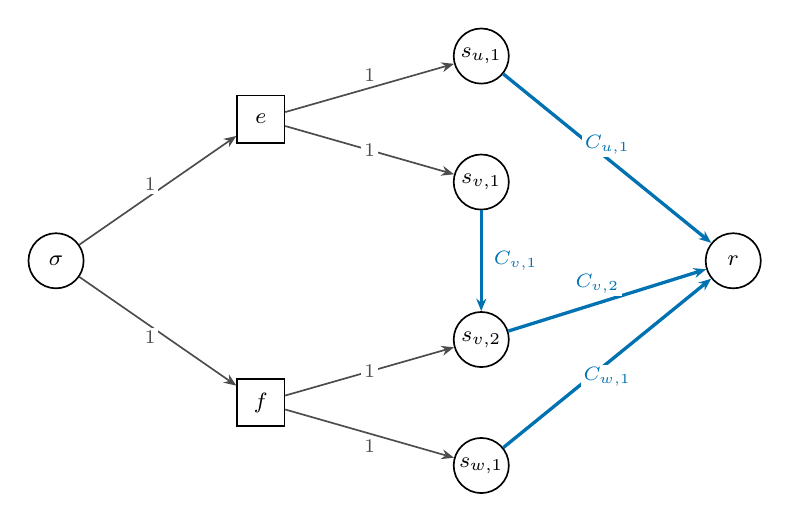
\begin{tikzpicture}[x=1cm,y=1cm,
  lbl/.style={font=\scriptsize,fill=white,inner sep=1pt},
  occ/.style={circle,draw,semithick,fill=white,minimum size=7mm,inner sep=0pt,font=\footnotesize},
  edg/.style={rectangle,draw,semithick,fill=white,minimum size=6mm,inner sep=0pt,font=\footnotesize},
  flow/.style={->,semithick,black!70},
  chain/.style={->,very thick,cA}]
  \node[circle,draw,semithick,fill=white,minimum size=7mm,inner sep=0pt,font=\footnotesize] (src) at (0,0) {$\sigma$};
  \node[edg] (e) at (2.6,1.8) {$e$};
  \node[edg] (f) at (2.6,-1.8) {$f$};
  \node[occ] (su1) at (5.4,2.6) {$s_{u,1}$};
  \node[occ] (sv1) at (5.4,1.0) {$s_{v,1}$};
  \node[occ] (sv2) at (5.4,-1.0) {$s_{v,2}$};
  \node[occ] (sw1) at (5.4,-2.6) {$s_{w,1}$};
  \node[occ] (r) at (8.6,0) {$r$};
  \draw[flow] (src) -- node[lbl,pos=0.45,yshift=4pt] {$1$} (e);
  \draw[flow] (src) -- node[lbl,pos=0.45,yshift=-4pt] {$1$} (f);
  \draw[flow] (e) -- node[lbl,pos=0.5,above=1pt] {$1$} (su1);
  \draw[flow] (e) -- node[lbl,pos=0.5] {$1$} (sv1);
  \draw[flow] (f) -- node[lbl,pos=0.5] {$1$} (sv2);
  \draw[flow] (f) -- node[lbl,pos=0.5,below=1pt] {$1$} (sw1);
  \draw[chain] (sv1) -- node[lbl,pos=0.5,right=3pt] {$C_{v,1}$} (sv2);
  \draw[chain] (sv2) -- node[lbl,pos=0.45,above=2pt] {$C_{v,2}$} (r);
  \draw[chain] (su1) -- node[lbl,pos=0.5,above=0pt] {$C_{u,1}$} (r);
  \draw[chain] (sw1) -- node[lbl,pos=0.5,below=0pt] {$C_{w,1}$} (r);
\end{tikzpicture}
\caption{Mạng chuỗi trên một ví dụ nhỏ. Đỉnh $v$ có hai lần xuất hiện, tại thời điểm của $e=\{u,v\}$ và tại thời điểm của $f=\{v,w\}$, trong đó $f$ là cạnh muộn hơn. Mỗi nút cạnh nhận một đơn vị từ nguồn $\sigma$ và gửi đơn vị đó đến nút lần xuất hiện của đầu mút được chọn làm đuôi. Cung rời khỏi $s_{v,j}$ có sức chứa $C_{v,j}$, và mọi chuỗi kết thúc tại đích $r$.}
\label{fig:chain}
\end{figure}


\begin{corollary}\label{cor:flow}
Nếu không có snapshot nào chứa thành phần chẵn, thì \FREE{} và \FIX{} được quyết định bởi một luồng cực đại trong mạng chuỗi. Trên mọi instance, một luồng cực đại có giá trị nhỏ hơn $m$ chứng nhận vô nghiệm.
\end{corollary}

\begin{proof}
Theo Định lý~\ref{thm:char} và Bổ đề~\ref{lem:noneven}, một định hướng là khả thi khi không có thành phần chẵn nào nếu và chỉ nếu nó thỏa mãn (i). Với \FIX{}, sau khi kiểm tra $\sum_va_v=\sum_vz_v$ và $h_v\in\N$ với mọi $v$, ta có $\sum_vh_v=m$, nên luồng có giá trị $m$ làm bão hòa mọi cung chuỗi cuối, cho $B_{v,q_v}=h_v$. Khẳng định thứ hai đúng vì (i) là điều kiện cần.
\end{proof}


Đồ thị thời gian proper không có thành phần chẵn, và trên chúng walk chặt và không chặt trùng nhau. Do đó Hệ quả~\ref{cor:flow} khôi phục Hệ quả~6.4 của Deligkas và cộng sự~\cite{deligkas2025} bằng một luồng cực đại và mở rộng nó cho \FREE{}.

Hình~\ref{fig:running} minh họa một thành phần chẵn chết. Hai walk xuất phát tại $x$ và $y$. Định hướng $x\to u\to y$ trong Hình~\ref{fig:running}(b) thỏa~(i) nhưng không để lại walk nào trong tam giác $u,v,w$ tại thời điểm~$2$, nên vi phạm~(ii). Cách sửa là đảo $u\to y$ tại thời điểm \emph{sớm hơn}~$1$ (Hình~\ref{fig:running}(c)).


\begin{figure}[htb]
\centering
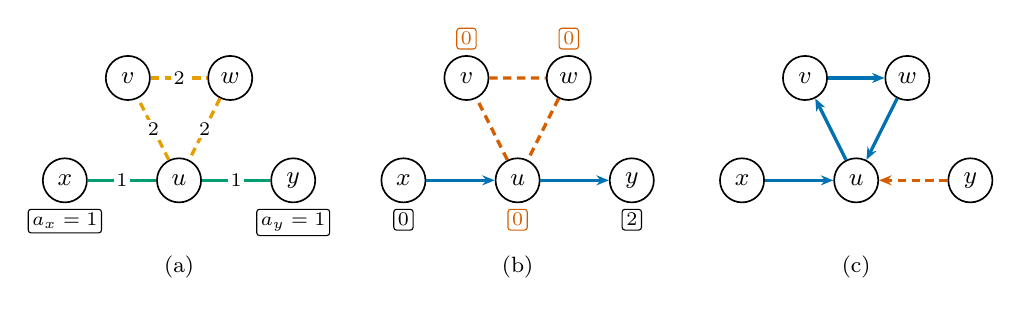
\begin{tikzpicture}
  \begin{scope}
    \RunningVertices
    \draw[t1] (x) -- node[tlab] {1} (u);
    \draw[t1] (u) -- node[tlab] {1} (y);
    \draw[t2] (u) -- node[tlab] {2} (v);
    \draw[t2] (v) -- node[tlab] {2} (w);
    \draw[t2] (w) -- node[tlab] {2} (u);
    \node[cnt,below=2pt of x] {$a_x=1$};
    \node[cnt,below=2pt of y] {$a_y=1$};
    \node[sub] at (1.45,-1.1) {(a)};
  \end{scope}
  \begin{scope}[xshift=4.3cm]
    \RunningVertices
    \draw[walkA] (x) -- (u);
    \draw[walkA] (u) -- (y);
    \draw[t2,cB] (u) -- (v) -- (w) -- (u);
    \node[cnt,below=2pt of x] {$0$};
    \node[cnt,draw=cB,text=cB,below=2pt of u] {$0$};
    \node[cnt,below=2pt of y] {$2$};
    \node[cnt,draw=cB,text=cB,above=2pt of v] {$0$};
    \node[cnt,draw=cB,text=cB,above=2pt of w] {$0$};
    \node[sub] at (1.45,-1.1) {(b)};
  \end{scope}
  \begin{scope}[xshift=8.6cm]
    \RunningVertices
    \draw[walkA] (x) -- (u);
    \draw[walkA] (u) -- (v);
    \draw[walkA] (v) -- (w);
    \draw[walkA] (w) -- (u);
    \draw[walkB] (y) -- (u);
    \node[sub] at (1.45,-1.1) {(c)};
  \end{scope}
\end{tikzpicture}
\caption{Ví dụ minh họa. (a) Nhãn thời gian và số lượng xuất phát. (b) Một định hướng thỏa mãn (i) với một tam giác chết. (c) Một lời giải với điểm kết thúc tự do.}
\label{fig:running}
\end{figure}

Phương pháp \emph{nhánh-cận khởi động lại} (\textbf{BB}) rẽ nhánh theo đỉnh của một thành phần chẵn chết được nhận thêm một cặp walk và tính lại luồng cực đại ở mỗi nhánh. Nó đúng, nhưng cây tìm kiếm của nó có thể có tới $2s^{e}$ nút với $e$ thành phần chẵn, mỗi thành phần có nhiều nhất $s$ đỉnh. Mục~\ref{sec:mconvex} và~\ref{sec:method} thay việc tìm kiếm này bằng các đường tăng. Mục~\ref{sec:counterexample} phân tích cách điều kiện (ii) bị mất trong phép quy tĩnh.


%% =====================================================================
\section{Phản ví dụ cho phép quy tĩnh}\label{sec:counterexample}

Mục này cho thấy phép quy tĩnh trong phác thảo chứng minh của Định lý~6.3 của~\cite{deligkas2025} không nắm bắt điều kiện (ii) của Định lý~\ref{thm:char}.

\paragraph{Phép quy.} Với một đỉnh $v$, gọi $\delta_{\le t}(v)$ và $\delta_{>t}(v)$ lần lượt là số cạnh kề với nó có nhãn thời gian không vượt quá $t$ và lớn hơn $t$. Chỉ số trên $G$ giới hạn các số đếm này ở các cạnh của $G$. Deligkas và cộng sự mở rộng mỗi đỉnh $v$ thành một dãy các bản sao $v_t$, một bản sao cho mỗi thời điểm mà $v$ có cạnh, và thêm một đầu cuối xuất phát $s$ và một đầu cuối kết thúc $e$. Hai bản sao liên tiếp được nối bởi $\alpha=\min(\delta_{\le t}(v),\delta_{>t}(v))$ cạnh, trong đó $\lceil\alpha/2\rceil$ cạnh có hướng về bản sao sau và phần còn lại là vô hướng: ``we create $\min(\delta_{\le t}(v),\delta_{\ge t+1}(v))$ edges between $v_t$ and $v_{t+1}$ \dots\ half of these edges rounded up are directed from $v_t$ to $v_{t+1}$, while the others are undirected''~\cite[tr.~26503]{deligkas2025}, xem thêm~\cite{deligkas2024arxiv}. Các cạnh vô hướng cho phép một walk tĩnh \emph{đi ngược thời gian}. Phác thảo chứng minh sửa một walk $W_1$ đi ngược thời gian bằng cách đổi đuôi với một walk khác $W_2$, vì ``there is at least one directed edge $(v_{t_i},v_{t_i+1})$ taken by some walk $W_2$ that entered to the left of $v_{t_i}$ and exits to the right''~\cite[tr.~26503--26504]{deligkas2025}. Lập luận này giả định $W_2\ne W_1$.


\begin{figure}[t]
\centering
\begin{tikzpicture}[stepn/.style={inner sep=1pt,font=\scriptsize}]
  \begin{scope}
    \node[vtx] (x) at (0,0) {$x$};
    \node[vtx] (u) at (1.3,0) {$u$};
    \node[vtx] (y) at (2.6,0) {$y$};
    \node[vtx] (v) at (0.7,1.2) {$v$};
    \node[vtx] (w) at (1.9,1.2) {$w$};
    \draw[t1] (x) -- node[tlab] {1} (u);
    \draw[t1] (u) -- node[tlab] {1} (y);
    \draw[t2] (u) -- node[tlab] {2} (v);
    \draw[t2] (v) -- node[tlab] {2} (w);
    \draw[t2] (w) -- node[tlab] {2} (u);
    \node[cnt,below=2pt of x] {$a_x=1$};
    \node[cnt,below=2pt of y] {$z_y=1$};
    \node[sub] at (1.3,-2.4) {(a)};
  \end{scope}
  \begin{scope}[xshift=4.8cm]
    \begin{scope}[on background layer]
      \foreach \t/\X in {0/0,1/1.5,2/3.4,3/5.3} {
        \draw[black!25,thin,densely dashed] (\X,2.0) -- (\X,-1.95);
        \node[note] at (\X,2.2) {$t=\t$};
      }
    \end{scope}
    \node[svtx] (s) at (-1.0,1.5) {$s$};
    \node[svtx] (x0) at (0,1.5) {$x_0$};
    \node[svtx] (x1) at (1.5,1.5) {$x_1$};
    \node[svtx] (u1) at (1.5,0) {$u_1$};
    \node[svtx] (u2) at (3.4,0) {$u_2$};
    \node[svtx] (v2) at (2.75,1.2) {$v_2$};
    \node[svtx] (w2) at (4.05,1.2) {$w_2$};
    \node[svtx] (y1) at (1.5,-1.5) {$y_1$};
    \node[svtx] (y3) at (5.3,-1.5) {$y_3$};
    \node[svtx] (e) at (6.3,-1.5) {$e$};
    \draw[walkA] (s) -- node[stepn,above] {1} (x0);
    \draw[walkA] (x0) -- node[stepn,above] {2} (x1);
    \draw[walkA] (x1) -- node[stepn,left] {3} (u1);
    \draw[walkA] (u1) to[bend left=20] node[stepn,above] {4} (u2);
    \draw[walkA] (u2) -- node[stepn,left=1.5pt,pos=0.6] {5} (v2);
    \draw[walkA] (v2) -- node[stepn,above,pos=0.3] {6} (w2);
    \draw[walkA] (w2) -- node[stepn,right=1.5pt,pos=0.4] {7} (u2);
    \draw[walkB] (u2) to[bend left=20] node[stepn,below,text=cB] {8} (u1);
    \draw[walkA] (u1) -- node[stepn,left] {9} (y1);
    \draw[walkA] (y1) -- node[stepn,below=1.5pt,pos=0.3] {10} (y3);
    \draw[walkA] (y3) -- node[stepn,below=1.5pt] {11} (e);
    \node[note,text=cB,anchor=north west] at (3.75,-0.2) {bước 8 quay lại\\thời gian};
    \node[sub] at (2.65,-2.4) {(b)};
  \end{scope}
\end{tikzpicture}
\caption{Phản ví dụ. (a) Instance thời gian. (b) Đồ thị tĩnh $S$ và một walk phủ nó.}
\label{fig:aaai}
\end{figure}

\begin{proposition}\label{prop:aaai}
Instance của Hình~\ref{fig:aaai}(a) không khả thi, nhưng đồ thị tĩnh $S$ của phép quy có một phủ chính xác cạnh với cùng số walk và cùng đầu cuối.
\end{proposition}


\begin{proof}
Instance có một walk, xuất phát tại $x$ và kết thúc tại $y$. Nó phải phủ cả hai cạnh tại thời điểm $1$ và kết thúc tại $y$, nên nó đi $x\to u\to y$. Sau đó không có walk nào nằm tại $u$, $v$ hay $w$, và tam giác vi phạm (ii) của Định lý~\ref{thm:char}. Trong $S$, xây dựng như trong phác thảo chứng minh của Định lý~6.3 của~\cite{deligkas2025} với đầu cuối $s$ nối vào $x$ tại thời điểm $0$ và $e$ nối vào $y$ tại thời điểm $3$ (Hình~\ref{fig:aaai}(b)), gadget của $u$ có $\alpha=\min(2,2)=2$ cạnh giữa $u_1$ và $u_2$, một cạnh có hướng $(u_1,u_2)$ và một cạnh vô hướng. Gadget của $x$ và $y$ mỗi cái có một cạnh có hướng. Walk tĩnh
\[
  s\to x_0\to x_1\to u_1\to u_2\to v_2\to w_2\to u_2\to u_1\to y_1\to y_3\to e
\]
phủ đúng một lần mọi cạnh của $S$, và bước $u_2\to u_1$ của nó (bước~8 trong Hình~\ref{fig:aaai}(b)) đi ngược từ thời điểm $2$ về thời điểm $1$. Nó là walk duy nhất, nên walk đi qua cạnh có hướng $(u_1,u_2)$ chính là $W_1$, và đổi đuôi với chính nó chỉ tách tam giác ra thành một chu trình không có walk.
\end{proof}


\begin{lemma}\label{lem:aaai}
Với \FIX{}, các cạnh vô hướng của $S$ có thể được định hướng sao cho mọi nút không đầu cuối cân bằng, với các cạnh đầu xuất phát hướng ra và các cạnh đầu kết thúc hướng vào, khi và chỉ khi có một định hướng của $G$ thỏa mãn điều kiện (i) của Định lý~\ref{thm:char} cùng với điều kiện cuối $B_{v,q_v}=h_v$.
\end{lemma}

\begin{proof}
Cố định một định hướng của $G$. Nó cũng định hướng các cạnh $\{u_t,v_t\}$ của $S$. Tại một đỉnh $v$, cạnh đầu xuất phát đóng góp $a_v$ cạnh vào trước nhãn thời gian đầu tiên, còn cạnh đầu kết thúc đóng góp $z_v$ cạnh ra sau nhãn thời gian cuối. Gọi $n_t$ là luồng ròng sang phải trên các cạnh nối sau bản sao $v_t$, và $n_{t^-}$ là đại lượng tương tự trước $v_t$. Cân bằng tại $v_t$ cho $n_t=n_{t^-}+\inn_t(v)-\out_t(v)$ với $n=0$ trước bản sao $v_0$ mà đầu xuất phát được gắn vào, nên theo quy nạp $n_t=c_{t^+}(v)$, và cân bằng tại bản sao cuối cho bộ đếm walk cuối $z_v$. Giữa hai nhãn thời gian liên tiếp có $\alpha_t=\min(\mathrm{before}_t,\mathrm{after}_t)$ cạnh với $\mathrm{before}_t=a_v+\delta^G_{\le t}(v)$ và $\mathrm{after}_t=z_v+\delta^G_{>t}(v)$. Trong số đó, $\lceil\alpha_t/2\rceil$ cạnh phải hướng sang phải, và các cạnh còn lại tự do. Các luồng ròng khả thi chính xác là các số nguyên $n$ với $n\equiv\alpha_t \pmod 2$ và $\alpha_t \bmod 2\le n\le\alpha_t$. Với $n=c_{t^+}(v)$, và dùng điều kiện cuối (bộ đếm walk cuối $z_v$), điều kiện chẵn lẻ luôn đúng, vì $c_{t^+}(v)$ có cùng tính chẵn lẻ với cả $\mathrm{before}_t$ và $\mathrm{after}_t$. Cận trên luôn đúng, vì $c_{t^+}(v)$ không vượt số cạnh vào đến thời điểm $t$ và không vượt số cạnh ra sau $t$. Cận dưới là $c_{t^+}(v)\ge0$, tức là điều kiện (i). Ngược lại, từ một định hướng thỏa mãn (i), ta chọn số cạnh tự do hướng sang phải sao cho $n_t=c_{t^+}(v)$, điều này khả thi vì giá trị này nằm trong khoảng cho phép.
\end{proof}


Bổ đề~\ref{lem:aaai} cho thấy rằng, với \FIX{}, đồ thị $S$ biểu diễn chính xác điều kiện (i) và điều kiện cuối, cùng với một điều kiện liên thông tĩnh (mọi thành phần của $S$ có cạnh đều chứa một đầu cuối). Nó không biểu diễn điều kiện (ii), vốn đòi hỏi một định hướng cho mọi thành phần chẵn một walk \emph{đồng thời}. Một lời giải thời gian luôn cho ra một phủ của $S$, và chiều ngược lại chỉ có thể sai do điều kiện (ii), như trong Mệnh đề~\ref{prop:aaai}. Khi chỉ đỉnh xuất phát được cho (\FREE{}), instance của Hình~\ref{fig:aaai}(a) không khả thi theo cùng lập luận.

Phản ví dụ gắn đầu cuối kết thúc tại một nhãn lớn hơn mọi nhãn, như trong Hình~3 của~\cite{deligkas2025}. Nếu câu ``for each terminal in $G$ connected to vertex $v$, we add a terminal in $S$ with an edge to $v_0$''~\cite[tr.~26503]{deligkas2025} được đọc theo nghĩa đen cho cả đầu cuối kết thúc, instance của Hình~\ref{fig:aaai} bị loại bỏ, nhưng phép quy khi đó loại bỏ cả các instance khả thi, chẳng hạn một cạnh duy nhất $\{0,1\}$ tại thời điểm~$2$ với $a=(0,1)$ và $z=(1,0)$, được giải bởi walk $1\to0$. Phân tích của chúng tôi dựa trên phiên bản AAAI và phiên bản~v1 của~\cite{deligkas2024arxiv}, và Mục~\ref{sec:exp-static} đo cả hai cách đọc trên các instance ngẫu nhiên và tổng hợp.

%% =====================================================================
\section{Tính M-lồi của các thành phần chẵn}\label{sec:mconvex}

Mục này chứng minh rằng tập trạng thái của một thành phần chẵn vẫn M-lồi sau khi bỏ trạng thái chết (Bổ đề~\ref{lem:gamma}(b)).

\subsection{Đếm theo cặp}

Viết $c_t(v)=2q_t(v)+p_t(v)$ với $p_t(v)\in\{0,1\}$ cố định và $q_t(v)$ là số \emph{cặp} walk tại $v$. Với một thành phần $K$ của $E_t$ và $v\in K$, đặt $p^{\inn}_v=p_t(v)$, $p^{\out}_v=p_{t^+}(v)$, $\alpha_v=q_t(v)$ (các cặp \emph{vào}) và $\beta_v=q_{t^+}(v)$ (các cặp \emph{ra}). Một định hướng của $K$ xác định hiệu $\beta-\alpha$ qua
\begin{equation}\label{eq:balance}
  \inn_t(v)-\out_t(v)=2(\beta_v-\alpha_v)+p^{\out}_v-p^{\inn}_v\qquad (v\in K).
\end{equation}
Ta nói $g\in\Z^K$ \emph{khả thực hiện} nếu có một định hướng của $K$ thỏa mãn~\eqref{eq:balance} với $g=\beta-\alpha$.

\begin{definition}\label{def:gamma}
Gọi $\Gamma_K\subseteq\Z^{K}\times\Z^{K}$ là tập các vector $(-\alpha,\beta)$ với $\alpha,\beta\ge0$ sao cho $\beta-\alpha$ khả thực hiện. Nếu $K$ chẵn, đặt $\Gamma'_K=\Gamma_K\setminus\{0\}$.
\end{definition}

Nếu $K$ chẵn, thì mọi bộ đếm walk trong $K$ đều chẵn trước và sau $t$, nên $c_t=2\alpha$ trên $K$. Lấy tổng~\eqref{eq:balance} trên $K$ cho $\beta(K)=\alpha(K)$, trong đó $x(X)=\sum_{i\in X}x_i$. Điều kiện (ii) tại $K$ do đó chính là $(-\alpha,\beta)\ne0$. Nói cách khác, \emph{một thành phần chẵn chết là trạng thái $0$ của gadget của nó}, và $\Gamma'_K$ là gadget với trạng thái này bị cấm.

\subsection{Công cụ từ lý thuyết lồi rời rạc}

Một tập $B\subseteq\Z^N$ là \emph{M-lồi}~\cite{murota2003} nếu với mọi $x,y\in B$ và mọi $i$ với $x_i>y_i$ tồn tại $j$ với $x_j<y_j$ sao cho $x-\e_i+\e_j\in B$ và $y+\e_i-\e_j\in B$. Bốn bổ đề sau từ lý thuyết định hướng~\cite{frank2011} và giải tích lồi rời rạc~\cite{murota2003,fujishige2005} được chứng minh ở đây cho cả các tập không bị chặn lẫn các tập bị chặn.

\begin{lemma}\label{lem:reversal}
Cho $O$ là một định hướng của $K$ thực hiện $g$, và $v\ne w$ là các đỉnh của $K$. Khi đó $g+\e_v-\e_w$ khả thực hiện khi và chỉ khi $O$ có một đường có hướng từ $v$ đến $w$.
\end{lemma}

\begin{proof}
Vì $\inn_t+\out_t$ là bậc cố định, \eqref{eq:balance} cho thấy thực hiện $g+\e_v-\e_w$ nghĩa là tăng bậc vào thêm một tại $v$, giảm một tại $w$ và giữ nguyên ở các đỉnh khác. Đảo một đường có hướng từ $v$ đến $w$ làm đúng điều này. Ngược lại, giả sử $O'$ thực hiện $g+\e_v-\e_w$ và gọi $H$ là tập các cung của $O$ bị đảo trong $O'$. Đảo cung $a\to b$ làm tăng bậc vào của $a$, nên $\out_H-\inn_H=\e_v-\e_w$. Gọi $Y$ là tập các đỉnh đi tới được từ $v$ trong $H$. Không có cung nào của $H$ đi ra khỏi $Y$, nên $\sum_{u\in Y}(\out_H(u)-\inn_H(u))\le0$. Vì $v\in Y$ đóng góp $1$, cũng có $w\in Y$, và $H\subseteq O$ chứa một đường có hướng từ $v$ đến $w$.
\end{proof}

\begin{lemma}\label{lem:boundary}
Cho $N$ là một mạng có hướng với sức chứa nguyên hoặc vô hạn, một tập $P$ các nút đầu cuối và các cung cấp \emph{cố định} nguyên tại mọi nút không đầu cuối. Tập các vector dòng vào ròng tại $P$ của các luồng nguyên khả thi trong $N$ là M-lồi khi nó khác rỗng. Tổng trực tiếp của các tập M-lồi là M-lồi.
\end{lemma}

\begin{proof}
Cho $f,f'$ là các luồng nguyên khả thi với vector dòng vào ròng $x,y$ tại $P$, và $x_i>y_i$. Gọi $D$ là đồ thị gồm $f(a)-f'(a)$ bản sao của mỗi cung $a$ có $f(a)>f'(a)$ và $f'(a)-f(a)$ bản sao của cung ngược của mỗi cung $a$ có $f(a)<f'(a)$. Dòng vào ròng của $D$ bằng $0$ tại các nút không đầu cuối và bằng $x_u-y_u$ tại mỗi nút đầu cuối $u$. Gọi $Y$ là tập các nút từ đó đi tới được $i$ trong $D$. Không có cung nào của $D$ đi vào $Y$, nên tổng dòng vào ròng của $D$ trên $Y$ không dương. Vì nó dương tại $i$, có một nút đầu cuối $j\in Y$ với $x_j<y_j$. Gọi $Q$ là một đường có hướng đơn từ $j$ đến $i$ trong $D$. Gửi một đơn vị dọc theo $Q$ chỉ thay đổi $f'$ trong phạm vi giữa $f$ và $f'$, giữ nguyên mọi cung cấp tại các nút không đầu cuối và cho vector dòng vào ròng $y+\e_i-\e_j$. Gửi một đơn vị ngược lại dọc theo $Q$ thay đổi $f$ theo cùng cách và cho $x-\e_i+\e_j$. Khẳng định về tổng trực tiếp suy ra từ định nghĩa, vì một phép trao đổi trong một hạng tử không làm thay đổi các hạng tử khác.
\end{proof}

\begin{lemma}\label{lem:exchange}
Cho $B$ là M-lồi, $x\in B$, và giả sử $x+\e_{i_l}-\e_{j_l}\in B$ với $l=1,\dots,r$, trong đó các $i_l$ đôi một khác nhau và các $j_l$ đôi một khác nhau. Nếu không có $l<l'$ nào mà $x+\e_{i_l}-\e_{j_{l'}}\in B$, thì $x+\sum_l(\e_{i_l}-\e_{j_l})\in B$.
\end{lemma}

\begin{proof}
Các cặp với $i_l=j_l$ không đóng góp gì và có thể bỏ đi. Giả thiết cùng với $x\in B$ cho $i_l\ne j_{l'}$ với $l<l'$. Ta quy nạp theo $r$, trường hợp $r\le1$ là hiển nhiên. Đặt $x'=x+\e_{i_r}-\e_{j_r}\in B$.

Trước hết cho $l<r$ và áp dụng tiên đề trao đổi cho $x+\e_{i_l}-\e_{j_l}$ và $x'$ tại tọa độ $i_l$, nơi điểm thứ nhất lớn hơn. Ta được $k\in\{j_l,i_r\}$, nơi điểm thứ nhất nhỏ hơn, với $x'+\e_{i_l}-\e_k\in B$. Nếu $k=i_r\ne j_l$ thì $x+\e_{i_l}-\e_{j_r}\in B$, điều mà giả thiết loại trừ. Do đó $x'+\e_{i_l}-\e_{j_l}\in B$.

Tiếp theo cho $l<l'<r$ và giả sử $u=x'+\e_{i_l}-\e_{j_{l'}}\in B$. Áp dụng tiên đề trao đổi cho $u$ và $x$ tại tọa độ $i_l$. Ta được $k\in\{j_{l'},j_r\}$ với $x+\e_{i_l}-\e_k\in B$, điều mà giả thiết loại trừ trong cả hai trường hợp. Do đó $x'+\e_{i_l}-\e_{j_{l'}}\notin B$.

Vậy các cặp $l<r$ thỏa giả thiết tại $x'$, và quy nạp cho khẳng định.
\end{proof}

\begin{lemma}\label{lem:localmax}
Cho $B$ là M-lồi, $x\in B$ và $R$ là một tập tọa độ. Nếu không có $i\in R$ và $j\notin R$ nào mà $x+\e_i-\e_j\in B$, thì $x(R)\ge y(R)$ với mọi $y\in B$.
\end{lemma}

\begin{proof}
Giả sử có $y\in B$ với $y(R)>x(R)$ và chọn $y$ như vậy với $\lVert y-x\rVert_1$ nhỏ nhất. Có $i\in R$ với $y_i>x_i$. Theo tiên đề trao đổi, có $j$ với $y_j<x_j$, $y-\e_i+\e_j\in B$ và $x+\e_i-\e_j\in B$. Giả thiết cho $j\in R$, nên $y'=y-\e_i+\e_j$ có $y'(R)=y(R)$ và gần $x$ hơn, mâu thuẫn.
\end{proof}

\subsection{Bổ đề chính}

Với $X\subseteq K$, gọi $\delta_K(X)$ là tập các cạnh của $K$ có đúng một đầu trong $X$.

\begin{lemma}\label{lem:gamma}
\begin{enumerate}
\item[(a)] $\Gamma_K$ là M-lồi.
\item[(b)] Nếu $K$ là một thành phần chẵn (liên thông), thì $\Gamma'_K=\Gamma_K\setminus\{0\}$ là M-lồi.
\end{enumerate}
\end{lemma}

\begin{proof}
(a) Cố định một định hướng tham chiếu $R$ của $K$ và đặt $d_R=\out-\inn$. Mọi định hướng khác được suy ra từ $R$ bằng cách đảo một tập cung, và đảo cung $x\to y$ chuyển một cặp từ $y$ sang $x$. Do đó $\beta-\alpha=\sigma+\partial\varphi$, trong đó $\sigma(v)=(p^{\inn}_v-p^{\out}_v-d_R(v))/2\in\Z$, $\varphi$ là vector $0/1$ trên các cung của đồ thị có hướng $R^-$ thu được bằng cách đảo mọi cung của $R$, và $\partial\varphi$ là dòng vào ròng của nó tại các đỉnh. Xây dựng mạng với, với mỗi $v$, một nút đầu cuối $v_{\inn}$ có cung không giới hạn $v_{\inn}\to v$ và một nút đầu cuối $v_{\out}$ có cung không giới hạn $v\to v_{\out}$, cùng với các cung của $R^-$ có sức chứa $1$ và cung cấp cố định $\sigma(v)$ tại mỗi nút $v$. Dòng vào ròng là $-\alpha_v$ tại $v_{\inn}$ và $\beta_v$ tại $v_{\out}$, nên $\Gamma_K$ là tập các vector đầu cuối của mạng này. Nó là M-lồi theo Bổ đề~\ref{lem:boundary}.

(b) Mọi tính chẵn lẻ trong một thành phần chẵn đều bằng $0$, nên \eqref{eq:balance} trở thành $\inn_t-\out_t=2g$ với $g=\beta-\alpha$. Ta dùng hai hệ quả. Thứ nhất, cho $O$ thực hiện $g$ và $\emptyset\ne X\subsetneq K$. Nếu mọi cạnh của $\delta_K(X)$ đi vào $X$ trong $O$ thì $g(X)=\abs{\delta_K(X)}/2>0$, và nếu mọi cạnh như vậy đi ra khỏi $X$ thì $g(X)<0$, vì $K$ liên thông. Thứ hai, mọi bậc trong $K$ đều chẵn, nên $K$ có chu trình Euler~\cite{hierholzer1873}. Định hướng thu được thực hiện $0$ và liên thông mạnh, nên $\e_v-\e_w$ khả thực hiện với mọi $v,w\in K$ theo Bổ đề~\ref{lem:reversal}.

Cho $x,y\in\Gamma'_K$ và $i$ là một tọa độ với $x_i>y_i$. Theo (a) có $j$ với $x_j<y_j$ sao cho $x'=x-\e_i+\e_j\in\Gamma_K$ và $y'=y+\e_i-\e_j\in\Gamma_K$. Nếu cả hai khác không thì xong. Chúng không thể đồng thời bằng không, vì khi đó $x=\e_i-\e_j=-y$, trong khi các tọa độ vào không dương và các tọa độ ra không âm, nên $i$ sẽ vừa là tọa độ ra ($x_i=1$) vừa là tọa độ vào ($y_i=-1$). Các điểm của $\Gamma_K$ thỏa $\alpha(K)=\beta(K)$, nên mọi điểm của $\Gamma'_K$ có $\alpha\ne0$ và $\beta\ne0$.

\emph{Trường hợp $x'=0$.} Khi đó $x=(-\e_u,\e_w)$, $i=w_{\out}$ và $j=u_{\inn}$. Viết $y=(-\alpha,\beta)$, đặt $g=\beta-\alpha$ và cho $O$ thực hiện $g$. Vì $y_i<1$, ta có $\beta_w=0$. Gọi $M$ là tập các đỉnh đi tới được từ $w$ trong $O$. Nếu $M\ne K$ thì mọi cạnh của $\delta_K(M)$ đi vào $M$, nên $\beta(M)\ge g(M)>0$. Nếu $M=K$ thì $\beta(K)\ge1$. Vậy có $z\in M\setminus\{w\}$ với $\beta_z\ge1$, và $g+\e_w-\e_z$ khả thực hiện theo Bổ đề~\ref{lem:reversal}. Lấy thay $j=z_{\out}$, thỏa $x_j=0<y_j$. Khi đó $x-\e_i+\e_j=(-\e_u,\e_z)\in\Gamma'_K$ theo hệ quả thứ hai, và $y+\e_i-\e_j\in\Gamma'_K$ vì hiệu của nó là $g+\e_w-\e_z$ và $\alpha\ne0$.

\emph{Trường hợp $y'=0$.} Khi đó $y=(-\e_u,\e_w)$, $i=u_{\inn}$ và $j=w_{\out}$. Viết $x=(-\alpha,\beta)$, đặt $g=\beta-\alpha$ và cho $O$ thực hiện $g$. Vì $x_i>-1$, ta có $\alpha_u=0$. Gọi $\Lambda$ là tập các đỉnh từ đó đi tới được $u$ trong $O$. Nếu $\Lambda\ne K$ thì mọi cạnh của $\delta_K(\Lambda)$ đi ra khỏi $\Lambda$, nên $\alpha(\Lambda)\ge-g(\Lambda)>0$. Nếu $\Lambda=K$ thì $\alpha(K)\ge1$. Vậy có $v\in\Lambda\setminus\{u\}$ với $\alpha_v\ge1$, và $g+\e_v-\e_u$ khả thực hiện theo Bổ đề~\ref{lem:reversal}. Lấy thay $j=v_{\inn}$, thỏa $x_j=-\alpha_v<0=y_j$. Khi đó $x-\e_i+\e_j$ chuyển một cặp vào từ $v$ sang $u$, hiệu của nó là $g+\e_v-\e_u$, và nó thuộc $\Gamma'_K$. Cuối cùng $y+\e_i-\e_j=(-\e_v,\e_w)\in\Gamma'_K$ theo hệ quả thứ hai.
\end{proof}

\begin{remark}\label{rem:connected}
Tính liên thông là cần thiết trong Bổ đề~\ref{lem:gamma}(b). Với hai tam giác rời nhau được coi là một thành phần duy nhất, tập tương ứng không là M-lồi. Phát biểu cũng nhạy với cách trình bày. Nếu $g=\beta-\alpha$ được cố định trước rồi điểm $0$ bị bỏ đi, tiên đề trao đổi đã thất bại ngay với hai đỉnh nối bằng hai cạnh song song. Vì vậy Bổ đề~\ref{lem:gamma}(b) được phát biểu cho $\Gamma'_K$ với $g$ tự do.
\end{remark}

%% =====================================================================
\section{Xây dựng luồng submodular và thuật toán}\label{sec:method}

Mục này dùng tính M-lồi trong Bổ đề~\ref{lem:gamma} để xây dựng một thuật toán thời gian đa thức cho \FREE{} và \FIX{}, trả về các walk hoặc một chứng nhận vô nghiệm (các Định lý~\ref{thm:reduction}, \ref{thm:correct} và~\ref{thm:time}).

\subsection{Mạng cổng}

Mỗi đỉnh $v$ trở thành một \emph{dòng thời gian} gồm các cổng. Gọi $K_1,\dots,K_{q_v}$ là các thành phần chứa các lần xuất hiện của $v$. Các cổng của $v$ là $S_v$ (bắt đầu), $\IN(K_j,v)$ và $\OUT(K_j,v)$ với $j=1,\dots,q_v$, và $Z_v$ (kết thúc). \emph{Các cung chờ} nối chúng theo thứ tự thời gian, cụ thể là $S_v\to\IN(K_1,v)$, $\OUT(K_j,v)\to\IN(K_{j+1},v)$ và $\OUT(K_{q_v},v)\to Z_v$. Một đỉnh không có cạnh chỉ có cung $S_v\to Z_v$. Một luồng $\xi\ge0$ trên một cung chờ là số cặp đang chờ tại $v$ giữa hai lần xuất hiện (Hình~\ref{fig:ports}). Với một cổng $P$, gọi $\partial\xi(P)$ là luồng ra khỏi $P$ trừ luồng vào $P$. Tại các cổng của một thành phần, $\partial\xi=(-\alpha,\beta)$.

Gọi $p_{\mathrm{end}}(v)$ là tính chẵn lẻ của $a_v+G_v$. Tập ràng buộc $\cB$ là tổng trực tiếp của các tập sau.
\begin{itemize}
\item Tại $S_v$, điểm duy nhất $\floor{a_v/2}$.
\item Tại các cổng của mỗi thành phần $K$, tập $\Gamma'_K$ nếu $K$ chẵn và $\Gamma_K$ trong trường hợp ngược lại.
\item Tại các cổng $Z_v$, với \FIX{}, điểm duy nhất $-(z_v-p_{\mathrm{end}}(v))/2$ tại mọi $v$, sau khi kiểm tra $z_v\equiv a_v+G_v \pmod 2$ và $z_v\ge p_{\mathrm{end}}(v)$. Với \FREE{}, đơn hình $\{-\gamma:\gamma\in\N^V,\ \gamma(V)=(k-\sum_vp_{\mathrm{end}}(v))/2\}$, chỉ cố định tổng số cặp cuối cùng.
\end{itemize}
Theo Bổ đề~\ref{lem:boundary} và~\ref{lem:gamma}, $\cB$ là M-lồi. Nó khác rỗng sau các kiểm tra ở dòng 1 của Thuật toán~\ref{alg:pf}. Vì $\sum_v(a_v+G_v)=k+2m$, số $k-\sum_vp_{\mathrm{end}}(v)$ luôn chẵn.

\begin{theorem}\label{thm:reduction}
Một instance của \FREE{} hoặc \FIX{} khả thi khi và chỉ khi có một luồng cặp $\xi\ge0$ trên các cung chờ với $\partial\xi\in\cB$.
\end{theorem}

\begin{proof}
($\Rightarrow$) Lấy định hướng của các walk và đặt $\xi=q$ trên mọi cung chờ. Tại $S_v$ ta có $\partial\xi=\floor{a_v/2}$. Tại mỗi thành phần, $\partial\xi=(-\alpha,\beta)$ với $\beta\ge0$ theo (i), hiệu $\beta-\alpha$ được chính định hướng đó thực hiện, và $(-\alpha,\beta)\ne0$ trên các thành phần chẵn theo (ii). Tại $Z_v$, giá trị $-\partial\xi$ là số cặp cuối cùng tại $v$. Nó bằng $(z_v-p_{\mathrm{end}}(v))/2$ trong \FIX{}, và trong \FREE{} các giá trị này có tổng $(k-\sum_vp_{\mathrm{end}}(v))/2$ vì số walk được bảo toàn.

($\Leftarrow$) Với mỗi $K$ chọn một định hướng thực hiện $\beta-\alpha$. Theo~\eqref{eq:balance}, số walk tại $v$ giữa hai lần xuất hiện dưới định hướng kết hợp bằng $2\xi+p$ trên cung chờ tương ứng. Điều kiện (i) đúng vì $\beta\ge0$. Điều kiện (ii) đúng trên các thành phần không chẵn theo Bổ đề~\ref{lem:noneven}, và trên các thành phần chẵn vì $(-\alpha,\beta)\ne0$. Với \FIX{}, số walk cuối cùng tại $v$ là $z_v$. Định lý~\ref{thm:char} hoàn tất chứng minh.
\end{proof}

\begin{figure}[t]
\centering
\begin{tikzpicture}[x=1.12cm,y=0.9cm,
  wait/.style={->,black!55,semithick},
  aug/.style={->,cA,line width=1.6pt},
  stp/.style={circle,fill=cA,text=white,font=\scriptsize\bfseries,inner sep=0.8pt,minimum size=3.4mm},
  hdr/.style={font=\scriptsize,text=black!70}]
  \def\cS{0} \def\cIa{1.7} \def\cOa{2.9} \def\cIb{4.9} \def\cOb{6.1} \def\cZ{7.9}
  \foreach \v/\Y in {x/2,y/1,u/0,v/-1,w/-2} {
    \node[font=\small] at (-0.55,\Y) {$\v$};
    \node[port] (S-\v) at (\cS,\Y) {};
    \node[port] (Z-\v) at (\cZ,\Y) {};
  }
  \foreach \v/\Y in {x/2,y/1,u/0} { \node[port] (I1-\v) at (\cIa,\Y) {}; \node[port] (O1-\v) at (\cOa,\Y) {}; }
  \foreach \v/\Y in {u/0,v/-1,w/-2} { \node[port] (I2-\v) at (\cIb,\Y) {}; \node[port] (O2-\v) at (\cOb,\Y) {}; }
  \begin{scope}[on background layer]
    \draw[cTa,semithick,rounded corners=2pt,fill=cTa!7] (\cIa-0.38,-0.42) rectangle (\cOa+0.38,2.42);
    \draw[cB,semithick,densely dashed,rounded corners=2pt,fill=cB!6] (\cIb-0.38,-2.42) rectangle (\cOb+0.38,0.42);
  \end{scope}
  \node[hdr] at (\cS,2.85) {$S_v$};
  \node[hdr] at (\cZ,2.85) {$Z_v$};
  \node[hdr] at (\cIa,2.85) {$\IN$};
  \node[hdr] at (\cOa,2.85) {$\OUT$};
  \node[hdr] at (\cIb,-2.85) {$\IN$};
  \node[hdr] at (\cOb,-2.85) {$\OUT$};
  \node[font=\scriptsize] at ({(\cIa+\cOa)/2},3.35) {thành phần tại thời điểm $1$: $\Gamma_K$};
  \node[font=\scriptsize] at ({(\cIb+\cOb)/2},-3.35) {thành phần tại thời điểm $2$: $\Gamma'_K$ (chẵn, chết)};
  \foreach \v in {x,y,u} \draw[wait] (S-\v) -- (I1-\v);
  \foreach \v in {v,w} \draw[wait] (S-\v) -- (I2-\v);
  \foreach \v in {x,y} \draw[wait] (O1-\v) -- (Z-\v);
  \draw[wait] (O1-u) -- (I2-u);
  \foreach \v in {u,v,w} \draw[wait] (O2-\v) -- (Z-\v);
  \node[circle,draw=black!55,fill=white,font=\scriptsize,inner sep=1pt] (eta) at (9.0,0.5) {$\eta$};
  \foreach \v in {x,y,u,v,w} \draw[black!40,thin,densely dashed] (Z-\v) -- (eta);
  \node[font=\scriptsize,above=1pt] at (7.0,1) {$\xi=1$};
  \node[font=\scriptsize,below=1pt] at (I2-u.south) {$+1$};
  \node[font=\scriptsize,below=1pt] at (O2-u.south) {$-1$};
  \draw[aug] ([yshift=-3pt]I2-u.west) -- node[stp,below=2pt] {1} ([yshift=-3pt]O1-u.east);
  \draw[aug] ([xshift=3pt]O1-u.north) -- node[stp,right=2pt] {2} ([xshift=3pt]O1-y.south);
  \draw[aug] ([yshift=-3pt]O1-y.east) -- node[stp,below=2pt,pos=0.86] {3} ([yshift=-3pt]Z-y.west);
  \draw[aug,-] (Z-y.east) -- (eta);
  \draw[aug] (eta) -- (Z-u.east);
  \node[stp] at ($(eta)+(0.45,0)$) {4};
  \draw[aug] ([yshift=-3pt]Z-u.west) -- node[stp,below=2pt] {5} ([yshift=-3pt]O2-u.east);
\end{tikzpicture}
\caption{Mạng cổng cho \FREE{} và một đường tăng sửa tam giác chết.}
\label{fig:ports}
\end{figure}

\subsection{Thuật toán đường tăng}\label{sec:auxgraph}

Thuật toán duy trì một luồng $\xi\ge0$ và một điểm $x\in\cB$. \emph{Độ lệch} $d=\partial\xi-x$ đo sự sai khác, và $d=0$ có nghĩa là đã tìm được lời giải. \emph{Đồ thị phụ} có các cổng làm nút và ba loại cung, mỗi cung chuyển một đơn vị độ lệch từ đuôi sang đầu.
\begin{enumerate}
\item[(1)] Đảo ngược của mọi cung chờ. Dùng nó làm tăng $\xi$ trên cung đó thêm một.
\item[(2)] Mọi cung chờ có $\xi>0$. Dùng nó làm giảm $\xi$ đi một.
\item[(3)] Một cung trao đổi $i\to j$ bất cứ khi nào $x+\e_i-\e_j\in\cB$. Dùng nó thay $x$ bằng $x+\e_i-\e_j$.
\end{enumerate}
Giả sử $i$ là một cổng của $v$ và $j$ là một cổng của $w$ trong cùng thành phần $K$. Cung trao đổi $i\to j$ tồn tại khi và chỉ khi $\alpha_v\ge1$ khi $i$ là cổng vào, $\beta_w\ge1$ khi $j$ là cổng ra, $v=w$ hoặc định hướng hiện tại của $K$ có một đường có hướng từ $v$ đến $w$ (Bổ đề~\ref{lem:reversal}), và nếu $K$ chẵn thì điểm mới khác không. Trong đơn hình của \FREE{}, $x+\e_i-\e_j\in\cB$ bất cứ khi nào $\gamma_i\ge1$. Thay vì $\Theta(n^2)$ cung này, đồ thị phụ chứa một nút $\eta$ với các cung $Z_i\to\eta$ với mọi $i$ có $\gamma_i\ge1$ và $\eta\to Z_j$ với mọi $j$, và một đường qua $\eta$ thực hiện một phép trao đổi đơn hình. Mọi kiểm tra đều thuần túy tổ hợp.

\begin{algorithm}[t]
\caption{Thuật toán đường tăng cho \FIX{} và \FREE{}}\label{alg:pf}
\begin{algorithmic}[1]
\State Kiểm tra các điều kiện đếm ($\sum a=\sum z$ và $h_v\in\N$ với \FIX{}, $k\ge\sum_vp_{\mathrm{end}}(v)$ với \FREE{}). \textbf{nếu} một kiểm tra thất bại \textbf{thì trả về} \NO{}.
\State Giải một luồng cực đại trong mạng chuỗi. \textbf{nếu} giá trị của nó nhỏ hơn $m$ \textbf{thì trả về} \NO{} cùng với lát cắt nhỏ nhất.
\State Lấy định hướng của luồng cực đại và $\xi$, $x$ cảm sinh. Với mỗi thành phần chẵn chết $K$, chọn $v\in K$, đặt $x=(-\e_v,\e_v)$ tại $(\IN(K,v),\OUT(K,v))$, để có $d=+1$ tại $\IN(K,v)$ và $d=-1$ tại $\OUT(K,v)$.
\While{tồn tại cổng có $d>0$}
  \State Tìm một đường \emph{ngắn nhất} từ $\{d>0\}$ đến $\{d<0\}$ trong đồ thị phụ bằng tìm kiếm theo chiều rộng.
  \If{không tồn tại đường như vậy}
    \State \Return \NO{} cùng với tập $R$ các cổng khả đạt từ $\{d>0\}$.
  \EndIf
  \State Áp dụng mọi cung của đường vào $\xi$ và $x$, và định hướng lại, bắt đầu từ định hướng hiện tại, các thành phần mà điểm của chúng đã thay đổi.
\EndWhile
\State \Return \YES{} và xây dựng các walk như trong chứng minh Định lý~\ref{thm:char}.
\end{algorithmic}
\end{algorithm}

Trong Hình~\ref{fig:ports}, các mũi tên đậm tạo thành một đường tăng sửa tam giác chết bằng cách đảo $u\to y$ tại thời điểm~$1$ và chuyển một điểm kết thúc từ $y$ sang $u$. Kết quả là lời giải của Hình~\ref{fig:running}(c).

\begin{example}\label{ex:fix}
Xét \FIX{} trên ví dụ minh họa với cả hai walk bắt buộc kết thúc tại $y$ ($z_y=2$). Không có nút $\eta$. Tìm kiếm theo chiều rộng từ $\IN(K,u)$, trong đó $K$ là tam giác tại thời điểm $2$, chỉ đạt $12$ cổng, và không cổng nào có $d<0$. Thuật toán trả về \NO{}, và $12$ cổng này tạo thành chứng nhận vô nghiệm.
\end{example}

\subsection{Tính đúng và các chứng nhận vô nghiệm}

\begin{lemma}\label{lem:invariant}
Sau mỗi lần tăng, $\xi\ge0$ và $x\in\cB$.
\end{lemma}

\begin{proof}
Mọi cung của đường được đánh giá tại trạng thái trước khi tăng và được áp dụng cùng lúc, nên các điểm trung gian không cần thuộc $\cB$. Một đường ngắn nhất là đơn, nên mỗi cung chờ được dùng nhiều nhất một lần và các cung loại~(2) chỉ được dùng khi $\xi>0$. Do đó $\xi\ge0$. Một đường đơn ghé $\eta$ nhiều nhất một lần, nên đơn hình của \FREE{} trải qua nhiều nhất một phép trao đổi, và phép này hợp lệ theo định nghĩa các cung. Xét một hạng tử khác $\Gamma$ của $\cB$ và các phép trao đổi $(i_1,j_1),\dots,(i_r,j_r)$ của nó theo thứ tự trên đường. Các nút của một đường ngắn nhất có khoảng cách theo chiều rộng đôi một khác nhau và tăng dần, nên các $i_l$ đôi một khác nhau và các $j_l$ đôi một khác nhau. Nếu tồn tại $l<l'$ với một cung $i_l\to j_{l'}$, thì $\mathrm{dist}(j_{l'})\le\mathrm{dist}(i_l)+1<\mathrm{dist}(i_{l'})+1=\mathrm{dist}(j_{l'})$, mâu thuẫn. Vậy giả thiết của Bổ đề~\ref{lem:exchange} được thỏa. Lập luận chỉ dùng thứ tự của các khoảng cách, nên không bị ảnh hưởng khi đường đi vào và rời cùng một thành phần nhiều lần. Ràng buộc $\ne0$ trên các thành phần chẵn cũng không gây khó khăn, vì bổ đề được áp dụng cho chính $\Gamma'_K$, là M-lồi theo Bổ đề~\ref{lem:gamma}. Theo Bổ đề~\ref{lem:exchange}, điểm mới vẫn nằm trong tập.
\end{proof}

\begin{theorem}\label{thm:correct}
Thuật toán~\ref{alg:pf} trả lời đúng. Khi nó trả lời \YES{}, các walk trả về tạo thành một lời giải. Khi nó trả lời \NO{} trong vòng lặp, tập $R$ các cổng khả đạt từ $\{d>0\}$ chứng nhận vô nghiệm.
\end{theorem}

\begin{proof}
\NO{} ở dòng~2 là đúng vì (i) là điều kiện cần. Tổng của $d$ trên mọi cổng luôn bằng $0$, nên nếu vòng lặp kết thúc thì $d=0$, và các walk được xây dựng qua Định lý~\ref{thm:reduction}. Giả sử thuật toán dừng với tập $R$. Nó chứa mọi cổng có $d>0$ và không chứa cổng nào có $d<0$, nên $d(R)>0$. Không có cung nào của đồ thị phụ rời khỏi $R$. Theo loại~(1), không có cung chờ nào đi vào $R$, và theo loại~(2), mọi cung chờ rời khỏi $R$ đều có $\xi=0$. Do đó $\partial\xi(R)=0$ và $x(R)=-d(R)<0$. Giả sử có một lời giải $(\xi',x')$ với $\xi'\ge0$ và $x'=\partial\xi'\in\cB$. Vì không có cung chờ nào đi vào $R$, $x'(R)$ là tổng của $\xi'$ trên các cung chờ rời khỏi $R$, nên $x'(R)\ge0$. Không có cung trao đổi nào rời khỏi $R$. Với đơn hình, điều này đúng vì một cổng $Z_i\in R$ với $\gamma_i\ge1$ đưa $\eta$ và mọi $Z_j$ vào $R$. Bổ đề~\ref{lem:localmax}, áp dụng cho từng hạng tử của tổng trực tiếp, cho $x(R)\ge x'(R)\ge0$, mâu thuẫn.
\end{proof}

Mọi câu trả lời \YES{} của cài đặt đều được chứng nhận, vì mọi walk trả về đều được kiểm tra theo định nghĩa. Câu trả lời \NO{} ở dòng~2 đi kèm một chứng nhận vô nghiệm dưới dạng một lát cắt của mạng chuỗi, có thể kiểm tra chỉ từ dữ liệu instance. Câu trả lời \NO{} từ vòng lặp không phụ thuộc Bổ đề~\ref{lem:exchange}, vì $x\in\cB$ được kiểm tra lúc chạy, nhưng nó vẫn phụ thuộc Bổ đề~\ref{lem:gamma} và~\ref{lem:localmax} và việc liệt kê đầy đủ các cung trao đổi. Chứng nhận vô nghiệm như vậy là \emph{phụ thuộc lý thuyết}.

\subsection{Độ phức tạp}

\begin{theorem}\label{thm:time}
Gọi $D$ là số thành phần chẵn chết sau luồng cực đại và $s$ là số đỉnh lớn nhất của một thành phần snapshot. Thuật toán~\ref{alg:pf} thực hiện nhiều nhất $D$ lần tăng và dùng
\[
  O\bigl(n+m\log(m+1)+m^2+D\,(n+s\,m)\bigr)\subseteq O(n+n\,m^2)
\]
phép toán số học, vì $D\le m/2$ và $s\le n$.
\end{theorem}

\begin{proof}
\emph{Số lần tăng.} Sau dòng~3, tổng các độ lệch dương bằng $D$. Mỗi lần tăng làm giảm $d$ đi một tại cổng đầu, tăng $d$ lên một tại cổng cuối, và để các cổng trong không đổi, nên tổng này giảm đúng một. Mỗi thành phần chẵn có ít nhất hai cạnh, nên $D\le m/2$.

\emph{Các dòng 1 đến 3.} Đọc dữ liệu và khởi tạo $n$ đỉnh mất $O(n)$. Sắp xếp các cạnh, xây dựng các snapshot và thành phần, và phát hiện thành phần chẵn mất $O(m\log(m+1))$. Mạng chuỗi có $O(m)$ nút và cung và giá trị luồng nhiều nhất $m$, nên phương pháp đường tăng mất $O(m^2)$.

\emph{Một lần tăng.} Số cổng là $2n+2Q\le2n+4m$, trong đó $Q\le2m$ là tổng số lần xuất hiện. Các cung loại~(1) và~(2) tốn $O(n+m)$. Với một thành phần $K$ có $m_K$ cạnh, các đỉnh khả đạt từ mỗi $v\in K$ được tìm bằng duyệt theo chiều sâu trong $O(\abs{K}m_K)$, và mỗi cổng có nhiều nhất $2\abs{K}$ cung trao đổi. Cộng trên mọi thành phần được $O(\sum_K\abs{K}m_K)\subseteq O(sm)$. Nút $\eta$ thêm $O(n)$. Một đường đơn dùng nhiều nhất $2\abs{K}$ cổng của $K$, nên vector bậc vào mới của $K$ khác vector cũ $O(\abs{K})$ đơn vị, và định hướng lại $K$ từ định hướng cũ cần $O(\abs{K})$ đường tăng mỗi đường tốn $O(m_K)$. Tổng cộng một lần tăng tốn $O(n+sm)$.
\end{proof}

Cận không phụ thuộc vào độ lớn của $a$ và $z$, và nó bao phủ cả quyết định. Liệt kê tường minh mọi $k$ walk tốn thêm $\Omega(k)$, đó là lý do chúng tôi xuất lời giải nén. Khi $D=0$ thuật toán chỉ là một luồng cực đại. Giá trị $D$ phụ thuộc vào luồng cực đại tìm được ở dòng~2, vì định hướng của bất kỳ lời giải nào cũng chính là một luồng cực đại với $D=0$. Với cài đặt của chúng tôi cho dòng~2, một họ các bản sao rời nhau của một gadget có năm đỉnh và bảy cạnh, mỗi bản sao giữ đúng một thành phần chẵn chết, cho $D=m/7$ với chín giá trị của $m$ từ $7$ đến $2.996$ ($D=428$ khi $m=2.996$). Với cài đặt này, cận $D\le m/2$ do đó đạt được tới một hệ số $3{,}5$. Đây không phải cận dưới cho tổng thời gian chạy.


\subsection{Cài đặt}\label{sec:impl}

Cài đặt của chúng tôi tính luồng cực đại ban đầu bằng cách xử lý các cạnh theo thứ tự thời gian tăng dần, gán đuôi một cách tham lam và tìm một đường tăng trong mạng dư ngay khi một cạnh không gán được. Tại thời điểm đó chỉ các cạnh sớm hơn đã được định hướng, nên việc tìm kiếm giữ được tính cục bộ trên dữ liệu thực. Đây là một thuật toán luồng cực đại, nên các kết quả về tính đúng không thay đổi, nhưng định hướng của nó, và do đó $D$, có thể khác với định hướng của thuật toán Dinic. Khác với phân tích của Định lý~\ref{thm:time}, cài đặt định hướng lại từ đầu bằng một luồng cực đại mỗi thành phần bị thay đổi bởi một lần tăng. Với cạnh song song, điều này tốn $O(n+m\log(m+1)+m^2+D(n+sm+\sum_Km_K^2))\subseteq O(n+nm+m^3)$ phép toán số học, trong đó tổng chạy trên các thành phần bị thay đổi bởi một lần tăng và $m_K$ là số cạnh của $K$. Mọi thời gian chạy được báo cáo đều dùng biến thể này.


\subsection{Các walk phải kết thúc trong một tập cho trước}

Gọi $\deg(v)$ là số cạnh tại $v$ trên mọi thời điểm và $\pi_v=(a_v+\deg(v))\bmod 2$.

\begin{proposition}\label{prop:parity}
Số walk kết thúc tại $v$ có tính chẵn lẻ của $a_v+\deg(v)$. Do đó một instance của \ENDSET{} không khả thi nếu $\pi_v=1$ với một $v\notin T$, nếu $a_v>0$ với một $v\notin T$ không có cạnh, hoặc nếu $\sum_{v\in T}\pi_v>k$.
\end{proposition}

\begin{proof}
Mỗi lần duyệt một cạnh tại $v$ làm thay đổi số walk nằm tại $v$ đúng một đơn vị, và có $\deg(v)$ lần duyệt như vậy. Một đỉnh không có cạnh giữ nguyên $a_v$ walk, và các walk này kết thúc tại đó. Khẳng định còn lại đúng vì tổng số walk kết thúc là $k$, và $k-\sum_{v\in T}\pi_v$ khi đó tự động chẵn.
\end{proof}

Viết số walk cuối cùng là $z_v=\pi_v+2\gamma_v$ với $\gamma_v\in\N$, trong đó $\gamma_v=0$ với $v\notin T$. Đặt $\Gamma_0=(k-\sum_{v\in T}\pi_v)/2$ và $P_T=\{-\gamma:\gamma\in\N^V,\ \gamma(V)=\Gamma_0,\ \gamma_v=0 \text{ với mọi } v\notin T\}$.

\begin{theorem}\label{thm:endset}
Sau kiểm tra của Mệnh đề~\ref{prop:parity}, \ENDSET{} được giải bởi Thuật toán~\ref{alg:pf} với tập $P_T$ tại các cổng $Z$ thay cho đơn hình của \FREE{}, và với thay đổi sau ở dòng~2. Với mỗi $v\notin T$, cung chuỗi cuối của $v$ nhận sức chứa và cận dưới $(a_v+\deg(v))/2$, để không walk nào kết thúc tại $v$. Cận thời gian của Định lý~\ref{thm:time} vẫn đúng.
\end{theorem}

\begin{proof}
Tập $P_T$ là M-lồi. Cho $x=-\gamma$ và $y=-\gamma'$ thuộc $P_T$ với $x_i>y_i$. Khi đó $\gamma_i<\gamma'_i$, nên $i\in T$. Vì $\gamma(V)=\gamma'(V)$, có $j$ với $\gamma_j>\gamma'_j\ge0$, nên $j\in T$. Các điểm $x-\e_i+\e_j=-(\gamma+\e_i-\e_j)$ và $y+\e_i-\e_j=-(\gamma'-\e_i+\e_j)$ thuộc $P_T$ vì $\gamma_j\ge1$ và $\gamma'_i\ge1$. Một luồng khả thi với các cận dưới này được tìm, hoặc chứng minh là không tồn tại, bằng một luồng cực đại bổ sung trong $O(m^2)$. Nếu không tồn tại, câu trả lời là \NO{}. Ngược lại nó cho một điểm ban đầu $x\in\cB$ với $P_T$ tại các cổng $Z$. Chứng minh Định lý~\ref{thm:reduction} chỉ dùng tổng số walk cuối và các tính chẵn lẻ $p_{\mathrm{end}}(v)=\pi_v$, nên nó đúng nguyên văn với $P_T$. Tổng trực tiếp của các tập M-lồi là M-lồi, nên Bổ đề~\ref{lem:invariant} và Định lý~\ref{thm:correct} áp dụng không đổi. Nút $\eta$ chỉ nối với các cổng $Z_v$ có $v\in T$, nên một lần tìm kiếm vẫn tốn $O(n)$ trên phần này.
\end{proof}

%% =====================================================================
\section{Walk chặt là NP-đầy đủ}\label{sec:strict}

Phủ chính xác cạnh bằng walk chặt là NP-đầy đủ khi số walk xuất phát được cho trước và các đỉnh kết thúc được cho trước hoặc tự do. Một walk \emph{chặt} có các nhãn thời gian tăng nghiêm ngặt và dùng nhiều nhất một cạnh của mỗi snapshot. Gọi \SFIX{} và \SFREE{} là các biến thể tương ứng của \FIX{} và \FREE{}. Trường hợp điểm kết thúc cho trước được Deligkas và cộng sự để mở~\cite[tr.~26504]{deligkas2025}, ngoài các trường hợp đặc biệt được điểm lại trong Mục~\ref{sec:related}.

\subsection{Các định hướng khả thi}

Một walk chặt đến một đỉnh tại thời điểm $t$ không thể rời đỉnh đó tại thời điểm $t$.

\begin{lemma}\label{lem:strict}
Một định hướng là khả thi bởi các walk chặt xuất phát theo $a$ khi và chỉ khi $\out_t(v)\le c_t(v)$ với mọi đỉnh $v$ và mọi thời điểm $t$. Với \SFIX{}, số walk cuối cùng tại $v$ còn phải bằng $z_v$ với mọi $v$.
\end{lemma}

\begin{proof}
\emph{Điều kiện cần.} Một walk chặt dùng nhiều nhất một cạnh tại thời điểm $t$. Vì vậy $\out_t(v)$ cung rời $v$ tại thời điểm $t$ được đi qua bởi các walk đôi một khác nhau, và mỗi walk trong số đó nằm tại $v$ ngay trước $t$. \emph{Điều kiện đủ.} Xử lý các thời điểm theo thứ tự tăng dần. Tại thời điểm $t$, gán cho các cung rời $v$ các walk đôi một khác nhau đang nằm tại $v$, điều này tồn tại vì $\out_t(v)\le c_t(v)$. Mỗi walk trong số này đi qua cung của nó, và mọi walk khác chờ. Số walk tại mọi đỉnh sau $t$ bằng $c_{t^+}$, nên quy nạp tiếp tục.
\end{proof}

So với Định lý~\ref{thm:char}, điều kiện (i) được thay bằng điều kiện mạnh hơn $\out_t(v)\le c_t(v)$, và điều kiện (ii) biến mất, vì mọi cạnh đều được đi qua bởi một walk đã ở đuôi của nó trước đó. Do đó một định hướng thỏa mãn điều kiện chặt không có thành phần chẵn chết. Theo các số $b_{v,j}$ và $B_{v,j}$ của Mục~\ref{sec:char}, điều kiện mới là $2B_{v,j-1}+b_{v,j}\le a_v+G_{v,j-1}$. Các tổng tiền tố rỗng bằng không. Các hệ số khác nhau của $b_{v,j}$ và $B_{v,j-1}$ khiến bất đẳng thức này không thể được biểu diễn bằng một ràng buộc sức chứa của mạng chuỗi.

\subsection{Phép quy}

Chúng tôi quy từ 3-SAT, bài toán thỏa mãn được Boolean với ba literal trên các biến khác nhau trong mỗi mệnh đề. Bước đầu của phép quy làm cho mỗi literal xuất hiện nhiều nhất hai lần; lớp bài toán thu được gần với lớp được Tovey nghiên cứu~\cite{tovey1984}. Trong một công thức mà mỗi mệnh đề có ba literal trên các biến khác nhau, thay $r\ge2$ lần xuất hiện của một biến $x$ bằng các biến mới $x_1,\dots,x_r$ và thêm các mệnh đề $(\lnot x_1\lor x_2),\dots,(\lnot x_{r-1}\lor x_r),(\lnot x_r\lor x_1)$, các mệnh đề này buộc $x_1,\dots,x_r$ bằng nhau. Khi đó mỗi literal của biến mới xuất hiện nhiều nhất hai lần: $x_j$ và $\lnot x_j$ mỗi cái xuất hiện một lần trong các mệnh đề thêm vào và nhiều nhất một lần trong các mệnh đề gốc.

Gọi $\varphi$ là một công thức như vậy với các biến $x_1,\dots,x_n$ và các mệnh đề $C_1,\dots,C_m$. Gọi $s_j\in\{2,3\}$ là số literal của $C_j$ và $d(\ell)\le2$ là số mệnh đề chứa literal $\ell$. Vì $\sum_js_j=\sum_\ell d(\ell)\le4n_\varphi$ và $s_j\ge2$, ta có $m_\varphi\le2n_\varphi$. Đồ thị thời gian $G_\varphi$ có một đỉnh cho mỗi trong $2n_\varphi$ literal, một đỉnh cho mỗi mệnh đề, một \emph{trung tâm} $h$, và các đỉnh bậc một gọi là \emph{lá}. Các cạnh của nó như sau (Hình~\ref{fig:strict}).
\begin{itemize}
\item \emph{Thời điểm $1$.} Một \emph{lá xuất phát} được nối với mỗi đỉnh literal, $s_j-1$ lá xuất phát được nối với $C_j$, và $4n_\varphi$ lá xuất phát được nối với $h$.
\item \emph{Thời điểm $2$.} Cạnh $\{x_i,\lnot x_i\}$ với mỗi biến $x_i$.
\item \emph{Thời điểm $3$.} Cạnh $\{C_j,\ell\}$ với mỗi mệnh đề $C_j$ và mỗi literal $\ell$ của $C_j$.
\item \emph{Thời điểm $4$ và $5$.} Một cạnh $\{\ell,h\}$ tại thời điểm $4$ và một cạnh tại thời điểm $5$, với mỗi đỉnh literal $\ell$.
\item \emph{Thời điểm $6$.} $d(\ell)$ \emph{lá kết thúc} được nối với mỗi đỉnh literal $\ell$, một lá kết thúc được nối với mỗi $C_j$, và $6n_\varphi-2m_\varphi$ lá kết thúc được nối với $h$.
\end{itemize}
Ta đặt $a_v=1$ tại mọi lá xuất phát, $z_v=1$ tại mọi lá kết thúc, và $a_v=z_v=0$ trong các trường hợp khác. Có $6n_\varphi+\sum_js_j-m_\varphi$ lá xuất phát và cũng bấy nhiêu lá kết thúc. Đồ thị $G_\varphi$ không có cạnh song song trong một snapshot, và kích thước của nó tuyến tính theo kích thước của $\varphi$. Hình~\ref{fig:strict} cho thấy các cạnh của nó tại một biến và một mệnh đề. Các cạnh từ $C_j$ đến các literal khác và các lá kết thúc của $\lnot x_i$ được lược bỏ ở đó. Nhãn cạnh là nhãn thời gian, và số bên cạnh một lá cho biết bội số của nó.

\begin{figure}[t]
\centering
\begin{tikzpicture}[
  lit/.style={circle,draw,semithick,fill=white,minimum size=6.4mm,inner sep=0pt,font=\footnotesize},
  leaf/.style={circle,draw,semithick,fill=white,minimum size=1.8mm,inner sep=0pt},
  eleaf/.style={circle,draw,semithick,fill=black!55,minimum size=1.8mm,inner sep=0pt},
  ed/.style={semithick},
  lab/.style={fill=white,inner sep=0.8pt,font=\scriptsize}]
  \node[lit] (x)  at (0,1.1)  {$x_i$};
  \node[lit] (nx) at (0,-1.1) {$\lnot x_i$};
  \node[lit] (c)  at (3.4,1.1) {$C_j$};
  \node[lit] (h)  at (3.4,-1.1) {$h$};
  \draw[ed] (x) -- node[lab] {2} (nx);
  \draw[ed] (x) -- node[lab] {3} (c);
  \draw[ed] (x) to[bend left=10] node[lab,pos=0.42] {4} (h);
  \draw[ed] (x) to[bend right=10] node[lab,pos=0.62] {5} (h);
  \draw[ed] (nx) to[bend left=12] node[lab] {4} (h);
  \draw[ed] (nx) to[bend right=12] node[lab] {5} (h);
  \node[leaf] (sx) at (-1.3,1.1) {};
  \node[leaf] (snx) at (-1.3,-1.1) {};
  \draw[ed] (sx) -- node[lab] {1} (x);
  \draw[ed] (snx) -- node[lab] {1} (nx);
  \node[eleaf] (ex) at (-0.9,2.1) {};
  \draw[ed] (x) -- node[lab] {6} (ex);
  \node[note,anchor=east] at (-1.05,2.1) {$d(x_i)$};
  \node[leaf] (sc) at (3.4,2.3) {};
  \draw[ed] (sc) -- node[lab] {1} (c);
  \node[note,anchor=west] at (3.55,2.3) {$s_j-1$};
  \node[eleaf] (ec) at (4.7,1.1) {};
  \draw[ed] (c) -- node[lab] {6} (ec);
  \node[leaf] (sh) at (4.7,-0.6) {};
  \draw[ed] (sh) -- node[lab] {1} (h);
  \node[note,anchor=west] at (4.85,-0.6) {$4n_\varphi$};
  \node[eleaf] (eh) at (4.7,-1.6) {};
  \draw[ed] (h) -- node[lab] {6} (eh);
  \node[note,anchor=west] at (4.85,-1.6) {$6n_\varphi-2m_\varphi$};
  \node[leaf] at (6.9,1.6) {};
  \node[note,anchor=west] at (7.05,1.6) {lá xuất phát ($a=1$)};
  \node[eleaf] at (6.9,1.1) {};
  \node[note,anchor=west] at (7.05,1.1) {lá kết thúc ($z=1$)};
\end{tikzpicture}
\caption{Đồ thị $G_\varphi$ quanh một biến $x_i$ và một mệnh đề $C_j$ chứa $x_i$.}
\label{fig:strict}
\end{figure}

\begin{theorem}\label{thm:strict}
\SFIX{} là NP-đầy đủ. Nó vẫn NP-đầy đủ khi đồ thị thời gian có sáu nhãn thời gian và không có cạnh song song trong một snapshot, và khi mọi đỉnh có $a_v+z_v>0$ đều là lá với $a_v+z_v=1$, nên mọi walk của mọi lời giải đều khác rỗng. \SFREE{} là NP-đầy đủ ngay cả với đồ thị thời gian có hai nhãn thời gian, và với ba nhãn thời gian nếu không cho phép walk rỗng.
\end{theorem}

\begin{proof}
Cả hai bài toán đều thuộc NP. Một định hướng là một chứng nhận được kiểm tra trong thời gian đa thức theo Bổ đề~\ref{lem:strict}; khi không cho phép walk rỗng, chứng nhận còn liệt kê các walk, số lượng nhiều nhất là $m_\varphi$, vì mỗi walk không rỗng dùng ít nhất một cạnh. Ta chứng minh $\varphi$ thỏa được khi và chỉ khi $G_\varphi$ cùng các vector $a$ và $z$ ở trên là một instance khả thi của \SFIX{}.

\emph{Một lời giải cho ra một phép gán thỏa mãn.} Lấy định hướng của một lời giải. Trước thời điểm $1$ chỉ các lá xuất phát giữ walk, nên điều kiện $\out_1(v)\le c_1(v)$ của Bổ đề~\ref{lem:strict} buộc mọi cạnh tại thời điểm $1$ hướng ra khỏi lá của nó. Trước thời điểm $2$ mọi đỉnh literal do đó giữ một walk, $C_j$ giữ $s_j-1$ walk và $h$ giữ $4n_\varphi$ walk. Cạnh $\{x_i,\lnot x_i\}$ tại thời điểm $2$ chuyển một walk, nên trước thời điểm $3$ một trong hai đỉnh $x_i$ và $\lnot x_i$ giữ hai walk và đỉnh kia không giữ walk nào. Gọi một literal là \emph{đúng} nếu đỉnh của nó giữ hai walk. Đúng một trong hai $x_i$ và $\lnot x_i$ là đúng, nên đây là một phép gán chân trị. Tại thời điểm $3$ đỉnh $C_j$ có $s_j$ cạnh nhưng chỉ giữ $s_j-1$ walk. Theo Bổ đề~\ref{lem:strict}, ít nhất một trong các cạnh này hướng từ một đỉnh literal $\ell$ đến $C_j$, và $\ell$ giữ một walk trước thời điểm $3$. Vậy $\ell$ đúng và $C_j$ được thỏa mãn.

\emph{Một phép gán thỏa mãn cho ra một lời giải.} Ta đưa ra một định hướng và kiểm tra Bổ đề~\ref{lem:strict}. Định hướng các cạnh tại thời điểm $1$ ra khỏi các lá, và cạnh $\{x_i,\lnot x_i\}$ từ literal sai đến literal đúng. Với mỗi mệnh đề $C_j$ chọn một literal đúng $\ell_j$ của $C_j$, định hướng $\{C_j,\ell_j\}$ từ $\ell_j$ đến $C_j$, và định hướng $s_j-1$ cạnh còn lại của $C_j$ ra khỏi $C_j$. Đỉnh $C_j$ dùng $s_j-1$ walk của nó. Một literal đúng $\ell$ được chọn bởi $\tau_\ell\le d(\ell)\le2$ mệnh đề và giữ hai walk, còn một literal sai không có cạnh ra. Sau thời điểm $3$, đỉnh $C_j$ giữ một walk, một literal sai $\ell$ giữ $d(\ell)$ walk, một literal đúng $\ell$ giữ $d(\ell)+2-2\tau_\ell$ walk, và $h$ giữ $4n_\varphi$ walk. Các cạnh tại thời điểm $4$ và $5$ đưa mọi đỉnh literal $\ell$ về đúng $d(\ell)$ walk.
\begin{itemize}
\item Nếu $\ell$ đúng và $\tau_\ell=0$, định hướng cả hai cạnh từ $\ell$ đến $h$. Đỉnh $\ell$ giữ $d(\ell)+2\ge2$ walk trước thời điểm $4$.
\item Nếu $\ell$ sai, hoặc đúng với $\tau_\ell=1$, định hướng cạnh tại thời điểm $4$ từ $h$ đến $\ell$ và cạnh tại thời điểm $5$ từ $\ell$ đến $h$. Đỉnh $\ell$ giữ ít nhất một walk trước thời điểm $5$.
\item Nếu $\ell$ đúng và $\tau_\ell=2$, định hướng cả hai cạnh từ $h$ đến $\ell$.
\end{itemize}
Tại mỗi thời điểm $4$ và $5$ có nhiều nhất $2n_\varphi$ cạnh rời $h$, và $h$ giữ $4n_\varphi$ walk trước thời điểm $4$ và ít nhất $2n_\varphi$ walk trước thời điểm $5$. Số walk tại $h$ thay đổi tổng cộng $\sum_{\ell\text{ đúng}}(2-2\tau_\ell)=2n_\varphi-2m_\varphi$, vì có $n_\varphi$ literal đúng và $\sum_\ell\tau_\ell=m_\varphi$. Do đó $h$ giữ $6n_\varphi-2m_\varphi\ge0$ walk trước thời điểm $6$, và ở đây $m_\varphi\le2n_\varphi$ được dùng. Trước thời điểm $6$ mọi đỉnh không phải lá do đó giữ đúng số walk bằng số lá kết thúc gắn vào nó, và các cạnh tại thời điểm $6$ hướng về các lá kết thúc. Số walk cuối cùng là $z$.

\emph{Đầu cuối tự do.} Chỉ giữ các đỉnh literal và đỉnh mệnh đề cùng các cạnh của thời điểm $2$ và $3$, và đặt $a_v=1$ tại mỗi đỉnh literal và $a_{C_j}=s_j-1$. Trước thời điểm $2$ mỗi đỉnh literal giữ một walk vì $a_v=1$, và mỗi đỉnh mệnh đề giữ $s_j-1$ walk. Các lập luận cho thời điểm $2$ và $3$ sau đó áp dụng không đổi, nên instance này của \SFREE{} khả thi khi và chỉ khi $\varphi$ thỏa được. Trong một lời giải, một literal đúng không được mệnh đề nào chọn giữ một walk rỗng. Nếu không cho phép walk rỗng, giữ thêm các lá xuất phát và các cạnh của thời điểm~$1$, với $a_v=1$ tại mỗi lá xuất phát và $a_v=0$ ở những nơi khác. Khi đó mọi walk bắt đầu bằng một cạnh, và các lập luận tương tự áp dụng với ba nhãn thời gian.
\end{proof}


\subsection{Thảo luận}

Đồ thị $G_\varphi$ không phải proper và các snapshot của nó có số cạnh khác nhau, nên Hệ quả~6.4 của~\cite{deligkas2025} không áp dụng, và Định lý~6.5 cũng không áp dụng: thời gian chạy của nó theo cấp số mũ theo $|V_S|$, và ở đây $|V_S|$ tăng theo $n_\varphi$; giả thiết $|E_t|\in\{0,k\}$ cũng bị vi phạm. Định lý~5.4 của~\cite{deligkas2025} xét bài toán không cho trước đỉnh xuất phát và không kéo theo Định lý~\ref{thm:strict}. Mọi đầu cuối trong phép xây dựng đều là một lá có bội số một, nên cũng thỏa mãn mô hình đầu cuối đa tập của~\cite{deligkas2025}. Kiểm tra bằng máy của phép quy được báo cáo ở Mục~\ref{sec:exp-correct}. Phép dựng dùng một hub có nhiều cạnh trong một snapshot, nên không giải quyết trường hợp mọi đỉnh có nhiều nhất hai cạnh trong mỗi snapshot, nằm giữa Hệ quả~6.4 của~\cite{deligkas2025} và Định lý~\ref{thm:strict}. Chúng tôi để mở trường hợp này.

%% =====================================================================
\section{Thực nghiệm tính toán}\label{sec:eval}

Các thực nghiệm phù hợp với tính đúng của cài đặt thuật toán luồng cặp (\textbf{PF}, Thuật toán~\ref{alg:pf}) và chỉ ra các lỗi của phép quy tĩnh. Các kiểm tra độc lập phù hợp với Định lý~\ref{thm:correct} (Mục~\ref{sec:exp-correct} và~\ref{sec:exp-even}). PF hoàn thành các bộ thử giao thông, tiếp xúc và tổng hợp, trong khi BB chạm giới hạn trên các instance lớn hơn (Mục~\ref{sec:exp-real} và~\ref{sec:exp-scale}). Phép quy tĩnh chấp nhận các instance vô nghiệm (Mục~\ref{sec:exp-static}).

\subsection{Cài đặt và instance}\label{sec:exp-setup}

Thiết kế bộ thử kiểm tra sự cần thiết của điều kiện~(ii) trong Định lý~\ref{thm:char} và hiệu năng của cài đặt ở Mục~\ref{sec:impl}. Các bản cài đặt độc lập của PF bằng Python và C++17 được so sánh với BB. Các bản cài đặt Python của PF và BB dùng cùng một backend max-flow.

\paragraph{Instance tổng hợp giàu thành phần chẵn.} Walk di chuyển theo cặp. Tại mỗi thời điểm, mỗi cặp hoạt động với xác suất $0{,}7$, và một cặp hoạt động hoặc đi qua một cạnh kép tới đỉnh khác (xác suất $0{,}25$), hoặc cho một walk của nó đi một chu trình độ dài $3$ đến $6$ qua đỉnh của nó (xác suất $0{,}3$), hoặc chuyển tới đỉnh khác theo hai đường đi rời nhau ở đỉnh trong, độ dài $1$ đến $3$ (xác suất $0{,}45$). Khi đó mỗi snapshot là hợp của các trail đóng, nên mọi bậc và mọi bộ đếm walk đều chẵn, và \emph{mọi} thành phần snapshot đều chẵn. Mọi thành phần cũng cân bằng, nên riêng điều kiện đếm chấp nhận mọi instance \FREE{}. Trong họ \emph{thưa}, đồ thị có khoảng $m/3$ đỉnh, nên các thành phần trong cùng một snapshot hiếm khi chạm nhau. Trong họ \emph{dày}, đồ thị có khoảng $2\sqrt m$ đỉnh, nên chúng thường gộp thành thành phần chẵn lớn hơn. Cả hai họ có khoảng $\sqrt m/2$ cặp. Nhãn đỉnh và thứ tự cạnh được xáo trộn, nên max-flow ban đầu không thấy định hướng đã cài sẵn. Mỗi đồ thị sinh ra cho bốn instance: \FIX{} và \FREE{} với các vector số walk xuất phát và kết thúc đã cài, khả thi theo cách dựng, và \FIX{} và \FREE{} bớt đi một cặp, chưa biết trước câu trả lời. Chúng tôi sinh $764$ đồ thị với $12\le m\le 20.000$, cho $3.056$ instance (Bảng~\ref{tab:even}). Các lượt chạy này thực hiện tuần tự trên Intel Core i9-9980HK chạy Linux, với Python~3.13.12 và backend mặc định của thư viện, không dùng SciPy.

\paragraph{Dữ liệu giao thông và tiếp xúc.} Chúng tôi cũng dựng instance từ lịch chạy một ngày của các mạng giao thông từ phiên bản~1.2 của bộ dữ liệu~\cite{kujala2018} (Zenodo record 1186215) và từ ba lớp của Copenhagen Networks Study (CNS)~\cite{sapiezynski2019}. Với tập điều tra của Mục~\ref{sec:exp-real}, mỗi bộ dữ liệu được cắt thành các cửa sổ thời gian nhiều độ dài (với giao thông là cửa sổ một giờ và, với Kuopio, Turku và Grenoble, cả ngày). Với dữ liệu giao thông, mỗi chuyến xe là một walk có các đoạn có phút khởi hành làm nhãn thời gian, và hướng cạnh bị bỏ qua. Tập điều tra và thực nghiệm C++ của Mục~\ref{sec:exp-scale} dùng các bộ nạp khác nhau (Kuopio có $987$ cạnh trong tập điều tra và $32.122$ cạnh trong thực nghiệm C++), nên hai tập giao thông không so sánh trực tiếp được. Dữ liệu tiếp xúc không ghi ai phụ trách sự kiện nào, nên số walk xuất phát được dựng bằng một quy tắc tham lam: duyệt các tiếp xúc theo thời gian, chuyển một walk qua mỗi tiếp xúc từ một đầu mút đang có walk, và tạo một walk mới tại đầu mút thứ nhất khi cả hai đều không có. Mỗi cửa sổ cho tối đa bốn instance: \FIX{} và \FREE{} khả thi theo cách dựng, và hai instance \FREE{} bỏ bớt một walk hoặc $10\%$ số walk (bỏ qua khi cửa sổ có quá ít walk). Tổng cộng có $18.250$ instance từ $4.639$ cửa sổ. Các lượt chạy tổng kê và giao thông chạy trên Intel Core i5-10210U (4 nhân) dưới Windows Subsystem for Linux thế hệ thứ hai (WSL2) với SciPy cho max-flow. Các thực nghiệm Python dùng Python~3.14.4 và SciPy~1.16.3, còn các thực nghiệm C++ dùng g++~15.2.0 và CMake~4.2.3. Hai đến bốn lượt trong số này chạy song song, nên thời gian có thể lệch khoảng hai lần.

\subsection{Tính đúng}\label{sec:exp-correct}

Các kiểm tra củng cố Định lý~\ref{thm:correct} bằng cách kiểm tra mọi câu trả lời \YES{} của PF theo định nghĩa walk và đối chiếu các câu trả lời với những bộ giải độc lập. Bảng~\ref{tab:checks} liệt kê các kiểm tra đối chiếu, gồm cả một kiểm tra bằng máy của phép quy ở Mục~\ref{sec:strict} với ba chương trình không dùng chung mã. Trên các instance nhỏ của kiểm tra oracle, có $5.494$ câu trả lời \NO{} trong vòng lặp tăng, nên phần này của thuật toán được thực thi. Kiểm tra bằng máy Bổ đề~\ref{lem:gamma} cũng xác nhận Nhận xét~\ref{rem:connected}. Tiên đề trao đổi sai với hai tam giác rời nhau, và sai ở $153$ trên $5.279$ tập gán nhãn khi cố định $g$ trước khi bỏ $0$, mỗi đồ thị chẵn trong $153$ đồ thị một lần.

\begin{table}[t]
\caption{Các kiểm tra tính đúng.}
\label{tab:checks}
\begin{tabular*}{\textwidth}{@{\extracolsep\fill}p{0.24\textwidth}p{0.38\textwidth}p{0.3\textwidth}}
\toprule
Kiểm tra & Quy mô & Kết quả \\
\midrule
Oracle vét cạn & $102.476$ instance nhỏ, mỗi instance giải cả \FIX{} và \FREE{} ($204.952$ lượt) & trùng khớp, $1.379$ lượt hoàn thành một bước tăng \\
PF và BB & $105.182$ lượt ($52.591$ instance cả \FIX{} và \FREE{}), tổng $1.840.950$ cạnh & trùng khớp \\
Instance giàu thành phần chẵn & $1.176$ lượt với $m\le14$ đối chiếu oracle, $2.960$ lượt với $m\le1.005$ đối chiếu BB & các lượt đã hoàn tất đều trùng khớp; BB dừng ở giới hạn trong $42$ lượt \\
Bổ đề~\ref{lem:gamma} & mọi đa đồ thị liên thông gán nhãn với $n\le5$, $m\le6$, hộp $0\le\alpha_v,\beta_v\le\deg(v)$ & không vi phạm trong $119.040$ tập $\Gamma_K$ và $153$ tập $\Gamma'_K$ \\
Các backend max-flow & $32.256$ instance, bốn bộ giải & trùng nhau về việc luồng có đạt $m$ \\
C++ và oracle & $378.040$ instance nhỏ & trùng khớp \\
Python và C++ & $8.000$ instance & trùng khớp \\
Phép quy chặt & $1.967$ công thức ($578$ không thỏa được, gồm cả $26$ công thức trên hai biến), instance \SFIX{} và \SFREE{} tới $156$ cạnh & tính khả thi luôn trùng tính thỏa được \\
\bottomrule
\end{tabular*}
\end{table}

Một chương trình riêng không import thư viện PF đã kiểm lại $13.028$ chứng nhận vô nghiệm từ ba tập instance. Từ $78{,}85\%$ đến $99{,}27\%$ chứng nhận ở mỗi tập là \emph{độc lập}, tức kiểm tra được chỉ từ dữ liệu instance, ví dụ dưới dạng một lát cắt của mạng chuỗi, và không instance \YES{} nào nhận chứng nhận vô nghiệm.

\subsection{Instance có nhiều thành phần chẵn}\label{sec:exp-even}

Bộ thử giàu thành phần chẵn tách riêng bước tăng của Thuật toán~\ref{alg:pf}: mọi thành phần snapshot đều chẵn, và max-flow ban đầu chấp nhận mọi instance (Bảng~\ref{tab:even}). Max-flow ban đầu để lại ít nhất một thành phần chẵn chết ở $1.349$ trên $3.056$ instance, và tỷ lệ thành phần chẵn chết trong số thành phần chẵn tăng theo kích thước, từ khoảng $8\%$ tại $m=12$ lên khoảng $63\%$ ở họ thưa tại $m=20.000$. Số thành phần chẵn chết lớn nhất là $D=3.310$. Trên mọi câu trả lời \YES{}, số bước tăng bằng đúng $D$, và cả $1.528$ instance cài sẵn đều được trả lời \YES{} với các walk qua được phép kiểm tra. Cả $449$ câu trả lời \NO{} đều xuất hiện khi vòng lặp tăng không tìm được đường tăng. Bớt một cặp làm $449$ trên $1.528$ instance bị bớt trở thành vô nghiệm.

\emph{Đồ thị}: số đồ thị sinh ra, mỗi đồ thị cho bốn instance. \emph{Chẵn}: số thành phần chẵn trung bình. \emph{Chết}: trung bình và lớn nhất của số thành phần chẵn chết $D$ sau max-flow ban đầu. \emph{Bớt}: số câu trả lời \YES{}/\NO{} của hai instance bớt một cặp. \emph{PF}: trung vị và lớn nhất của thời gian (giây). \emph{BB}: số lượt dừng ở giới hạn $2.000$ max-flow hoặc $10$ giây ($5$ giây với $m=1.000$) trên tổng số lượt. \emph{Tĩnh}: số instance \FIX{} được quy tắc của Mục~\ref{sec:exp-static} chấp nhận trên số instance \FIX{} vô nghiệm. Dấu gạch nghĩa là không chạy.

\begin{table}[t]
\caption{Bộ thử tổng hợp giàu thành phần chẵn. Mỗi ô ghi $a/b$. \textbf{Even}: số thành phần chẵn trung bình trên mỗi đồ thị. \textbf{Dead}: trung bình/lớn nhất số thành phần chẵn chết còn lại sau luồng cực đại ban đầu. \textbf{Cut}: số đáp án YES/NO của PF trên các instance đã bỏ một cặp. \textbf{PF}: trung vị/lớn nhất thời gian chạy tính bằng giây. \textbf{BB}: số lần dừng ở giới hạn thời gian / tổng số lần chạy BB. \textbf{Static}: số instance mà quy tắc tĩnh trả YES trong khi PF trả NO, trên tổng số instance PF trả NO mà quy tắc được chạy. Dấu gạch ngang nghĩa là phương pháp không được chạy.}
\label{tab:even}
\footnotesize
\begin{tabular*}{\textwidth}{@{\extracolsep\fill}lrrrrrrrr}
\toprule
Họ & $m$ & Đồ thị & Chẵn & Chết & Bớt & PF & BB & Tĩnh \\
\midrule
thưa & $12$ & $200$ & $3{,}0$ & $0{,}3$/$4$ & $265$/$135$ & $<0{,}001$/$<0{,}001$ & $0$/$800$ & $77$/$78$ \\
dày & $12$ & $200$ & $2{,}7$ & $0{,}3$/$4$ & $280$/$120$ & $<0{,}001$/$<0{,}001$ & $0$/$800$ & $72$/$72$ \\
thưa & $50$ & $100$ & $7{,}4$ & $0{,}7$/$5$ & $165$/$35$ & $<0{,}001$/$0{,}002$ & $0$/$400$ & $23$/$23$ \\
dày & $50$ & $100$ & $7{,}1$ & $0{,}6$/$4$ & $172$/$28$ & $<0{,}001$/$0{,}002$ & $0$/$400$ & $19$/$19$ \\
thưa & $200$ & $50$ & $35{,}9$ & $10{,}0$/$24$ & $50$/$50$ & $0{,}007$/$0{,}014$ & $10$/$200$ & $28$/$28$ \\
dày & $200$ & $50$ & $21{,}9$ & $3{,}4$/$12$ & $83$/$17$ & $0{,}004$/$0{,}011$ & $2$/$200$ & $11$/$11$ \\
thưa & $1.000$ & $20$ & $218{,}8$ & $90{,}8$/$117$ & $3$/$37$ & $0{,}157$/$0{,}215$ & $30$/$80$ & $20$/$20$ \\
dày & $1.000$ & $20$ & $78{,}4$ & $16{,}1$/$27$ & $40$/$0$ & $0{,}079$/$0{,}132$ & $0$/$80$ & $0$/$0$ \\
thưa & $5.000$ & $10$ & $1242{,}1$ & $682{,}3$/$733$ & $0$/$20$ & $4{,}81$/$7{,}29$ & -- & -- \\
dày & $5.000$ & $10$ & $305{,}1$ & $77{,}5$/$94$ & $19$/$1$ & $1{,}74$/$2{,}20$ & -- & -- \\
thưa & $20.000$ & $2$ & $5183{,}5$ & $3277{,}6$/$3.310$ & $0$/$4$ & $154{,}8$/$170{,}5$ & -- & -- \\
dày & $20.000$ & $2$ & $1098{,}5$ & $309{,}5$/$315$ & $2$/$2$ & $51{,}3$/$56{,}8$ & -- & -- \\
\bottomrule
\end{tabular*}
\end{table}

\subsection{Dữ liệu giao thông và tiếp xúc}\label{sec:exp-real}

Tập điều tra giao thông và tiếp xúc kiểm tra tần suất trở ngại trong Định lý~\ref{thm:char}(ii) đòi hỏi bước tăng (Bảng~\ref{tab:census}). Thành phần chẵn xuất hiện thường xuyên trên lịch chạy giao thông, nơi $224$ trên $316$ instance của tập điều tra có thành phần chẵn, và trên lớp Bluetooth của Copenhagen Networks Study ($4.788$ trên $13.552$). Các lớp cuộc gọi và tin nhắn không có. Tập điều tra dùng phép gán tham lam rồi thuật toán Dinic cho max-flow ban đầu, còn các thực nghiệm C++ dùng bộ giải theo thời gian của Mục~\ref{sec:impl}. Trong $304$ instance giao thông dựng từ cửa sổ một giờ có $2$ instance có thành phần chẵn chết, còn trong $12$ instance dựng từ lịch chạy cả ngày có $6$. Trên các lịch chạy lớn hơn của thực nghiệm C++ ở Mục~\ref{sec:exp-scale}, $48$ trên $50$ instance còn thành phần chẵn chết sau max-flow ban đầu, với $D$ tới $467$. Trên dữ liệu tiếp xúc với vector số walk xuất phát dựng tham lam, chỉ $11$ trên $17.934$ instance có thành phần chẵn chết. Trên mọi instance \YES{}, số bước tăng của PF bằng đúng $D$, và mọi câu trả lời \NO{} trên dữ liệu thực đến từ max-flow.

\emph{Chẵn}: số instance có thành phần chẵn. \emph{Chết}: số instance mà max-flow để lại thành phần chẵn chết. \emph{Tăng}: số bước tăng lớn nhất. \emph{Giây}: thời gian lớn nhất của PF.

\begin{table}[t]
\caption{Điều tra trên $18.250$ instance từ dữ liệu giao thông và tiếp xúc.}
\label{tab:census}
\begin{tabular*}{\textwidth}{@{\extracolsep\fill}lrrrrrrr}
\toprule
Nguồn & Inst. & $m$ lớn nhất & Chẵn & Chết & Tăng & \YES{}/\NO{} & Giây \\
\midrule
Kuopio & $52$ & $987$ & $8$ & $0$ & $0$ & $31$/$21$ & $0{,}0$ \\
Turku & $88$ & $125.779$ & $80$ & $5$ & $316$ & $49$/$39$ & $83{,}2$ \\
Grenoble & $92$ & $52.710$ & $60$ & $3$ & $44$ & $50$/$42$ & $4{,}3$ \\
Adelaide & $84$ & $7.681$ & $76$ & $0$ & $0$ & $45$/$39$ & $0{,}3$ \\
CNS Bluetooth & $13.552$ & $25.222$ & $4.788$ & $11$ & $1$ & $7.968$/$5.584$ & $1{,}1$ \\
CNS cuộc gọi & $1.994$ & $3.599$ & $0$ & $0$ & $0$ & $1.098$/$896$ & $0{,}1$ \\
CNS tin nhắn & $2.388$ & $24.260$ & $0$ & $0$ & $0$ & $1.261$/$1.127$ & $1{,}1$ \\
\midrule
Tổng & $18.250$ & & $5.012$ & $19$ & & $10.502$/$7.748$ & \\
\bottomrule
\end{tabular*}
\end{table}

\subsection{Thời gian chạy}\label{sec:exp-scale}

Thời gian chạy cho thấy hiệu năng thực tế của cài đặt ở Mục~\ref{sec:impl} và sự tăng trưởng của BB trên họ thiếu cặp.

\paragraph{Instance giàu thành phần chẵn.} Trên bộ thử giàu thành phần chẵn, thời gian trung vị của PF dưới $0{,}2$ giây cho tới $m=1.000$ và là $4{,}8$ giây tại $m=5.000$, nơi có tới $D=733$ thành phần chẵn chết được sửa. Các instance lớn nhất, với $m=20.000$, mất tối đa $170$ giây. BB, giới hạn $2.000$ max-flow và vài giây mỗi instance, bị dừng ở $30$ trên $80$ lượt của họ thưa tại $m=1.000$, nơi $D$ trung bình khoảng $90$.

\paragraph{Một họ thiếu cặp cho BB.} Một đỉnh trung tâm $h$ giữ $e-1$ cặp walk. Khối $i$ gồm hai cạnh kép từ $h$ tại thời điểm $2i-1$ rồi một tam giác tại thời điểm $2i$, với $i=1,\dots,e$. Mỗi tam giác cần một cặp nên instance vô nghiệm, nhưng không khối đơn lẻ nào cho thấy sự thiếu hụt. Bảng~\ref{tab:family} cho thấy BB tăng gấp đôi số max-flow sau mỗi khối ($87.167$ max-flow tại $e=16$) và không giải xong $e=17$ trong phần ngân sách thời gian còn lại là $96$ giây. PF cần khoảng $e/4$ bước tăng và giải $e=2.000$ ($14.000$ cạnh) trong $106$ giây. Họ này được thiết kế để bộc lộ các trường hợp khó cho BB.

Mọi instance đều vô nghiệm. Lượt chạy có tổng ngân sách $270$ giây, và BB bị dừng tại $e=17$ khi hết ngân sách. Thời gian dưới $0{,}01$ giây chủ yếu là nhiễu.

\begin{figure}[t]
\centering
\begin{tikzpicture}
\begin{loglogaxis}[width=0.9\textwidth,height=6.8cm,
  xlabel={$e$ (số khối)},ylabel={thời gian chạy (s)},
  xmin=1.5,xmax=3000,ymin=0.0001,ymax=300,
  grid=major,grid style={black!10},
  legend style={at={(0.5,-0.26)},anchor=north,legend columns=3,draw=none,column sep=10pt},legend cell align=left,
  mark size=2pt,
  every axis plot/.append style={thick}]
\addplot[color=cA,mark=*,only marks] coordinates {
(2,0.0002) (3,0.0004) (4,0.0004) (5,0.0005) (6,0.0006) (7,0.0007) (8,0.0007) (9,0.0016) (10,0.0028) (11,0.0043) (12,0.0019) (13,0.0023) (14,0.0057) (15,0.0029) (16,0.0099) (17,0.0029) (18,0.0036) (19,0.0036)
(20,0.0042) (50,0.024) (100,0.0945) (200,0.4014) (500,2.7615) (1000,11.9697) (2000,105.7992)};
\addlegendentry{PF}
\addplot[color=cB,mark=square*,only marks] coordinates {
(2,0.0017) (3,0.012) (4,0.0164) (5,0.0289) (6,0.0854) (7,0.1469) (8,0.4175) (9,0.8466) (10,1.7191) (11,3.7738) (12,8.4594) (13,18.1987) (14,21.0141) (15,35.3492) (16,83.4539)};
\addlegendentry{BB}
\addplot[color=cB,mark=square,only marks,mark options={fill=white}] coordinates {(17,96.4369)};
\addlegendentry{BB, stopped (lower bound)}
\addplot[color=cA,dashed,no markers,domain=2:2000,samples=2] {0.0000002*x^2} node[pos=0.85,above,font=\scriptsize,color=cA] {$\propto e^2$};
\end{loglogaxis}
\end{tikzpicture}
\caption{Thời gian chạy của PF và BB trên họ thiếu cặp, theo thang log-log. Mỗi điểm là một instance với $e$ khối; ô vuông rỗng đánh dấu lượt chạy BB bị dừng khi hết giới hạn thời gian, nên giá trị của nó là cận dưới. Đường đứt là đường tham chiếu có độ dốc hai, không phải đường khớp. Các thời gian dưới $0{,}01$ giây chủ yếu là nhiễu, và mỗi giá trị đến từ một lần chạy.}
\label{fig:scale}
\end{figure}

Hình~\ref{fig:scale} vẽ cùng số đo trên thang log-log.

\begin{table}[t]
\caption{Thời gian chạy (giây) trên họ thiếu cặp.}
\label{tab:family}
\begin{tabular*}{\textwidth}{@{\extracolsep\fill}lrrrrrrrr}
\toprule
$e$ & $2$ & $4$ & $8$ & $12$ & $16$ & $17$ & $100$ & $2.000$ \\
\midrule
BB & $0{,}0017$ & $0{,}0164$ & $0{,}418$ & $8{,}46$ & $83{,}5$ & vượt & & \\
PF & $0{,}0002$ & $0{,}0004$ & $0{,}0007$ & $0{,}0019$ & $0{,}0099$ & $0{,}0029$ & $0{,}095$ & $105{,}8$ \\
\bottomrule
\end{tabular*}
\end{table}

\paragraph{Lịch chạy giao thông.} Trên lịch chạy cả ngày của Turku ($125.779$ cạnh), PF giải \FIX{} trong $70{,}3$ giây và \FREE{} trong $33{,}7$ giây, còn BB không xong trong $150$ giây.

\paragraph{C++ trên 25 mạng giao thông.} Bản C++17 (g++ 15.2, chế độ Release, WSL2) dùng max-flow theo thời gian của Mục~\ref{sec:impl} và qua các dòng C++ của Bảng~\ref{tab:checks}. Chúng tôi chạy nó trên cả $25$ thành phố của bộ dữ liệu, với \FIX{} và \FREE{} cho mỗi thành phố. Với $13$ thành phố chúng tôi dùng lịch chạy cả ngày. Với $12$ mạng còn lại (Adelaide, Berlin, Brisbane, Dublin, Helsinki, Lisbon, Melbourne, Paris, Prague, Rome, Sydney và Winnipeg) chúng tôi chỉ giữ các chuyến bắt đầu trong khối ba giờ đông nhất trong ngày. Cả $50$ instance được trả lời \YES{}, và các walk được dựng và kiểm tra bởi mã C++. Ở $48$ instance, max-flow ban đầu để lại thành phần chẵn chết, và $D$ lớn nhất là $467$. PF mất từ $0{,}7$ đến $79$ giây mỗi instance (trung vị $13{,}9$ giây), gồm $68{,}7$ giây cho instance lớn nhất, Paris \FIX{} với $387.467$ cạnh và $D=287$. Bản C++ của BB, giới hạn $2.000$ max-flow và $2$ giây, chạm giới hạn ở $48$ instance, nên chỉ $2$ instance được đối chiếu với nó.

Trên các bộ thử, PF hoàn thành mọi lượt chạy, đạt tới $387.467$ cạnh trên dữ liệu giao thông và $D=3.310$ thành phần chẵn chết trên dữ liệu tổng hợp.

\subsection{Độ chính xác của phép quy tĩnh}\label{sec:exp-static}

Các phép kiểm tra xác nhận rằng phép quy tĩnh có thể chấp nhận các instance thời gian vô nghiệm, như Mệnh đề~\ref{prop:aaai} khẳng định, và đối chiếu các ràng buộc định hướng của nó với Bổ đề~\ref{lem:aaai}.

\paragraph{Instance ngẫu nhiên.} Trên $20.000$ instance \FIX{} nhỏ ngẫu nhiên (hạt giống $20261030$, $n\le5$, $m\le7$, ba nhãn thời gian), mọi lời giải thời gian đều cho một $S$ khả thi. Một định hướng cân bằng của $S$ tồn tại khi và chỉ khi có một định hướng thỏa mãn (i) và các số walk cuối cho trước, như Bổ đề~\ref{lem:aaai} dự đoán. Có $52$ instance mà $S$ khả thi nhưng instance thời gian vô nghiệm, và ở $9$ instance điều kiện (i) đúng nhưng $S$ không khả thi do điều kiện liên thông tĩnh. Với cách đọc đúng từng chữ, cùng các instance này cho $5$ câu trả lời \YES{} sai và $3.778$ câu trả lời \NO{} sai, nên kết luận phụ thuộc vào cách đọc phép dựng.

\paragraph{Instance giàu thành phần chẵn.} Trên các instance \FIX{} của bộ thử giàu thành phần chẵn với $m\le1.005$, chúng tôi chạy quy tắc ``nếu $S$ có định hướng cân bằng và mọi thành phần chạm một terminal thì trả lời \YES{}'', theo cách đọc của Hình~3 trong~\cite{deligkas2025}. Quy tắc này chấp nhận $250$ trên $251$ instance vô nghiệm. Trong đó có $121$ trên $122$ instance mà oracle vét cạn chứng minh vô nghiệm và $233$ trên $234$ instance mà BB chứng minh vô nghiệm. Nó không bao giờ bác một instance khả thi. Một bộ thử trước đó trên một họ tam giác rời nhau và trên các bản sao của phản ví dụ cho bức tranh tương tự. Hai bộ giải bất đồng ở $160$ trên $437$ instance, và trong cả $160$ ca quy tắc chấp nhận một instance mà PF bác. Vét cạn xác nhận PF ở $40$ ca đủ nhỏ trong số đó.

Do đó quy tắc dựa trên Hình~3 của~\cite{deligkas2025} chủ yếu sai khi điều kiện~(ii) quyết định tính vô nghiệm trong các instance giàu thành phần chẵn đã thử.

\subsection{Phạm vi và giới hạn}\label{sec:scope}

Mô hình giao thông bỏ qua hướng cạnh, thời gian di chuyển giữa các chuyến, ca làm việc và bến xe, nên không xác lập tính khả thi vận hành của các ca xe. Các instance giao thông chưa chỉnh sửa khả thi theo cách dựng. Bộ sinh giàu thành phần chẵn và số walk xuất phát tham lam cho dữ liệu tiếp xúc hạn chế các phân phối instance, còn họ thiếu cặp không cho biết tần suất các trường hợp khó cho BB. Số thành phần chẵn chết $D$ được đo với một max-flow ban đầu cho mỗi bộ dữ liệu. BB là baseline duy nhất, chưa có so sánh với các mô hình quy hoạch nguyên hay thỏa mãn được Boolean. Thời gian chạy được đo trên hai máy, một phần với các lượt chạy song song, nên khả năng so sánh trực tiếp thời gian bị hạn chế.

%% =====================================================================
\section{Kết luận}\label{sec:conclusion}

Phủ chính xác cạnh bằng walk thời gian không chặt với số walk xuất phát cho trước có một mô hình luồng submodular M-lồi và một thuật toán đường tăng thời gian đa thức kèm chứng nhận vô nghiệm. Mô hình dựa trên tính M-lồi của một thành phần chẵn sau khi bỏ trạng thái chết của nó, một điều kiện mà phép quy tĩnh không biểu diễn. Phủ chính xác cạnh bằng walk chặt là NP-đầy đủ, ngay cả khi điểm kết thúc được cho trước. Các giới hạn của thực nghiệm được tóm tắt ở Mục~\ref{sec:scope}. Công việc tương lai bao gồm các cận cho bài toán NP-khó cực tiểu hóa số walk khi các đỉnh xuất phát tự do, độ phức tạp của walk chặt khi mỗi đỉnh có nhiều nhất hai cạnh trong mỗi snapshot, và sự phụ thuộc của số thành phần chẵn chết vào luồng cực đại ban đầu.

\backmatter

\bmhead{Lời cảm ơn}
Chúng tôi cảm ơn các tác giả của~\cite{deligkas2025} về những trao đổi hữu ích liên quan đến phản ví dụ. Các tác giả đã dùng một trợ lý AI (Claude, Anthropic) để dịch và chỉnh sửa ngôn ngữ cho bản thảo này. Các tác giả đã kiểm tra văn bản thu được và chịu trách nhiệm đầy đủ về nội dung.

\section*{Khai báo}

\begin{itemize}
\item \textbf{Tài trợ} Các tác giả không nhận được hỗ trợ từ bất kỳ tổ chức nào cho công trình này.
\item \textbf{Xung đột lợi ích} Các tác giả tuyên bố không có xung đột lợi ích.
\item \textbf{Phê duyệt đạo đức và đồng ý tham gia} Không áp dụng.
\item \textbf{Đồng ý xuất bản} Không áp dụng.
\item \textbf{Khả dụng dữ liệu} Dữ liệu Copenhagen Networks Study~\cite{sapiezynski2019} và dữ liệu giao thông~\cite{kujala2018} có sẵn từ các nhà cung cấp theo điều khoản của họ. Bộ sinh instance tổng hợp và tóm tắt kết quả thô có tại https://github.com/th1enq/exact-edge-cover-temporal-walks. Dữ liệu thô không được phân phối lại; các instance có thể tái tạo bằng các script trong kho.
\item \textbf{Khả dụng vật liệu} Không áp dụng.
\item \textbf{Khả dụng mã nguồn} Thư viện Python, bản C++17 và các script thực nghiệm có tại https://github.com/th1enq/exact-edge-cover-temporal-walks.
\item \textbf{Đóng góp của tác giả} D.T.Q.: Ý tưởng (Conceptualization), phương pháp (Methodology), phân tích hình thức (Formal analysis), phần mềm (Software), điều tra (Investigation), thẩm định (Validation), viết bản thảo gốc (Writing – original draft). M.C.T.: giám sát (Supervision), viết lại và chỉnh sửa (Writing – review \& editing); M.C.T. là tác giả liên hệ. Tất cả tác giả đã đọc và phê duyệt bản thảo cuối cùng.
\end{itemize}

\bibliography{references}

\end{document}

